\documentclass[aspectratio=169,11pt]{beamer}

\usepackage[utf8]{inputenc}
\usepackage[T1]{fontenc}
\usepackage{lmodern}
\usepackage{amsmath,amssymb,amsfonts}
\usepackage{mathtools}
\usepackage{booktabs}
\usepackage{graphicx}
\usepackage{tikz}
\usetikzlibrary{positioning,arrows.meta,calc}
\usepackage{ragged2e}
\usepackage{hyperref}
\usepackage{array}

\usetheme{default}
\useinnertheme{rectangles}

\definecolor{AcademicBlue}{RGB}{24,55,95}
\definecolor{SoftBlue}{RGB}{232,239,247}
\definecolor{DarkGray}{RGB}{55,55,55}
\definecolor{SolutionGreen}{RGB}{42,112,78}
\definecolor{SoftGreen}{RGB}{232,245,238}
\usetikzlibrary{arrows.meta,calc,angles,quotes}
\definecolor{VectorPurple}{RGB}{103,73,151}
\definecolor{DarkGray}{RGB}{55,55,55}
\definecolor{AxisGray}{RGB}{130,140,150}

\setbeamercolor{normal text}{fg=DarkGray,bg=white}
\setbeamercolor{structure}{fg=AcademicBlue}
\setbeamercolor{frametitle}{fg=AcademicBlue,bg=white}
\setbeamercolor{title}{fg=AcademicBlue}
\setbeamercolor{subtitle}{fg=DarkGray}
\setbeamercolor{block title}{fg=white,bg=AcademicBlue}
\setbeamercolor{block body}{fg=DarkGray,bg=SoftBlue}
\setbeamercolor{alerted text}{fg=AcademicBlue}
\setbeamercolor{example text}{fg=SolutionGreen}
\setbeamercolor{block title example}{fg=white,bg=SolutionGreen}
\setbeamercolor{block body example}{fg=DarkGray,bg=SoftGreen}

\setbeamerfont{title}{size=\LARGE,series=\bfseries}
\setbeamerfont{subtitle}{size=\normalsize}
\setbeamerfont{author}{size=\normalsize}
\setbeamerfont{institute}{size=\small}
\setbeamerfont{frametitle}{size=\large,series=\bfseries}
\setbeamerfont{block title}{series=\bfseries}
\setbeamersize{text margin left=0.55cm,text margin right=0.55cm}
\setbeamertemplate{navigation symbols}{}

\newcommand{\frontlogos}{%
    
\includegraphics[height=1.05cm]{logo-its.png}\hspace{0.22cm}%
    
\includegraphics[height=0.82cm]{logo-advancing-humanity.png}\hspace{0.22cm}%
    
\includegraphics[height=0.95cm]{logo-m.png}%
}

\newcommand{\slideMlogo}{%
    
\includegraphics[height=0.72cm]{logo-m.png}%
}

\newcommand{\source}[1]{%
    \vfill
    \hfill{\tiny\color{gray}Sumber: #1}
}

\newcommand{\axisgrid}[4]{%
    \draw[step=1cm,gray!20,very thin] (#1,#3) grid (#2,#4);
    \draw[-{Latex[length=2mm]},AcademicBlue,thick] (#1,0)--({#2+0.25},0) node[right] {$x$};
    \draw[-{Latex[length=2mm]},AcademicBlue,thick] (0,#3)--(0,{#4+0.25}) node[above] {$y$};
}

\setbeamertemplate{headline}{}

\setbeamertemplate{frametitle}{
    \vspace{0.15cm}
    \noindent\hbox to \textwidth{%
        \begin{minipage}[c]{0.86\textwidth}
            \raggedright
            \usebeamerfont{frametitle}
            \usebeamercolor[fg]{frametitle}
            \insertframetitle
        \end{minipage}%
        \hfill
        \begin{minipage}[c]{0.08\textwidth}
            \raggedleft
            \slideMlogo
        \end{minipage}%
    }
    \vspace{-0.05cm}
    {\color{AcademicBlue}\rule{\textwidth}{0.6pt}}
    \vspace{0.15cm}
}

\setbeamertemplate{footline}{
    \leavevmode
    \hbox{%
        \begin{beamercolorbox}[
            wd=.75\paperwidth,
            ht=2.8ex,
            dp=1.2ex,
            leftskip=0.5cm
        ]{normal text}
        \scriptsize \insertshorttitle
        \end{beamercolorbox}%
        \begin{beamercolorbox}[
            wd=.25\paperwidth,
            ht=2.8ex,
            dp=1.2ex,
            rightskip=0.5cm plus1fil
        ]{normal text}
        \hfill\scriptsize \insertframenumber/\inserttotalframenumber
        \end{beamercolorbox}%
    }
}

\setbeamertemplate{itemize item}{\color{AcademicBlue}\small$\blacksquare$}
\setbeamertemplate{itemize subitem}{\color{AcademicBlue}\scriptsize$\blacktriangleright$}

\AtBeginSection[]{
    \begin{frame}
        \vfill
        \begin{center}
            {\color{AcademicBlue}\Large\bfseries \insertsection}
            \vspace{0.3cm}

            {\color{AcademicBlue}\rule{0.35\textwidth}{0.8pt}}
        \end{center}
        \vfill
    \end{frame}
}


\usetikzlibrary{automata,patterns}
\newcommand{\eps}{\varepsilon}
\newcommand{\D}{\mathcal{M}_{\mathrm{in}}^{\mathrm{ax}}[[\gamma,\delta]]}
\newcommand{\mpmat}[1]{\begin{pmatrix}#1\end{pmatrix}}
\newcommand{\res}{\mathbin{\backslash\!\circ}}
\tikzset{tr/.style={rectangle,draw=AcademicBlue,fill=AcademicBlue,minimum width=2mm,minimum height=8mm},
pl/.style={circle,draw=AcademicBlue,thick,minimum size=8mm},
ar/.style={-{Latex},thick,AcademicBlue}}

\newcommand{\N}{\mathbb N}
\newcommand{\Pre}{\mathrm{Pre}}
\newcommand{\Post}{\mathrm{Post}}
\newcommand{\tok}[1]{\fill[AcademicBlue] (#1.center) circle (2.2pt);}
\tikzset{tall/.style={tr,minimum height=11mm},state/.style={draw=AcademicBlue,rounded corners,fill=SoftBlue,inner sep=4pt}}

\title[Kapita Selekta Aljabar -- Systems in Dioids]{Kapita Selekta Aljabar}
\subtitle{Petri Net, Timed Event Graph, dan Aljabar Gamma--Delta}
\author{}
\institute{Program Studi S1 Matematika\\Institut Teknologi Sepuluh Nopember}
\date{Systems in Dioids}
\begin{document}


% 1
\begin{frame}[plain]
    \vspace{0.15cm}
    \begin{flushleft}
        \frontlogos
    \end{flushleft}
    \vspace{0.50cm}
    {\color{AcademicBlue}\rule{\textwidth}{1.2pt}}
    \vspace{0.50cm}

    {\usebeamerfont{title}\color{AcademicBlue}\inserttitle\par}
    \vspace{0.25cm}
    {\usebeamerfont{subtitle}\insertsubtitle\par}
    \vspace{0.50cm}

    {\usebeamerfont{author}\textbf{\insertauthor}\par}
    \vspace{0.15cm}
    {\usebeamerfont{institute}\insertinstitute\par}
    \vspace{0.35cm}
    {\small\insertdate}
    \vfill
\end{frame}

\begin{frame}{Peta materi}

\begin{enumerate}
\item Petri net: struktur, marking, enabling, dan firing.
\item Event graph serta perluasan dengan waktu.
\item Dioid, max-plus, matriks, dan analisis jadwal.
\item Deret formal serta aljabar $\gamma$--$\delta$.
\item Kleene star dan hubungan masukan--keluaran.
\item Residuasi, kendali just-in-time, filter, dan umpan balik.
\item Studi kasus serta latihan dengan pembahasan.
\end{enumerate}
Setiap konsep diawali interpretasi, lalu definisi dan contoh hitungan.

\end{frame}
\begin{frame}{Sumber dan konvensi pembelajaran}

Sumber utama adalah Part III buku \textit{Control of Discrete-Event Systems:
Automata and Petri Net Perspectives} (2013).
\begin{itemize}
\item Bab 21: pemodelan dan analisis sistem dalam dioid.
\item Bab 22: teori dan sintesis kendali.
\item \S16.2.2 memperjelas istilah timed dan time Petri net.
\end{itemize}
Nomor halaman rujukan mengikuti halaman cetak buku.
\begin{block}{Prasyarat}
Himpunan, fungsi, operasi biner, dan matriks dasar.
Monoid, urutan parsial, serta deret formal dijelaskan dalam materi.
\end{block}

\end{frame}
\begin{frame}{Kapan sebuah kegiatan dapat dimulai?}


Dua komponen siap pada waktu $4$ dan $7$. Perakitan membutuhkan keduanya.
\[
t_{\mathrm{mulai}}=\max(4,7)=7.
\]
Jika perakitan memerlukan $3$ satuan waktu:
\[
t_{\mathrm{selesai}}=\max(4,7)+3=10.
\]
\begin{block}{Dua operasi yang muncul}
Sinkronisasi menggunakan maksimum. Durasi menambahkan waktu.
\end{block}
Contoh sederhana disusun untuk kuliah, mengikuti motivasi Bab 21.

\source{Bab 21, hlm. 431--450}

\end{frame}
\begin{frame}{Petri net}
\begin{center}{\LARGE\bfseries\color{AcademicBlue}Petri net}\\[8mm]Struktur graf, token, dan perubahan keadaan\end{center}
\end{frame}
\begin{frame}{Sistem kejadian diskrit}

Sistem kejadian diskrit berubah ketika suatu \textbf{kejadian} berlangsung.
\begin{center}\begin{tabular}{ll}\toprule
Konteks&Contoh kejadian\\\midrule
Mesin produksi&Pekerjaan mulai atau selesai\\
Transportasi&Kereta berangkat atau tiba\\
Komputasi&Proses memperoleh atau melepas sumber daya\\\bottomrule
\end{tabular}\end{center}
Keadaan dapat mencatat ketersediaan barang atau sumber daya.
\begin{block}{Contoh mesin}
Sumber daya bebas dapat diambil suatu pekerjaan,
lalu dikembalikan ketika pekerjaan selesai.
\end{block}
Petri net memodelkan kondisi dan kejadian secara terpisah.

\source{\S21.1, hlm. 431--434; contoh kuliah}
\end{frame}
\begin{frame}{Komponen grafis Petri net}

\begin{center}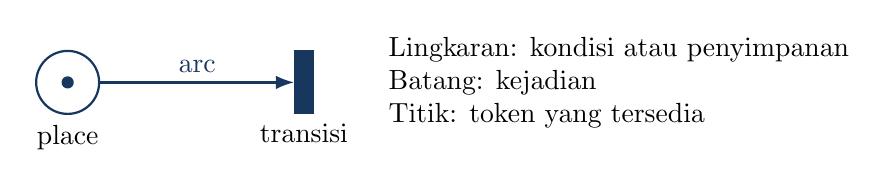
\begin{tikzpicture}
\node[pl,label=below:place] (p) at (0,0) {};
\tok{p}
\node[tr,label=below:transisi] (t) at (3,0) {};
\draw[ar] (p)--node[above]{arc}(t);
\node[align=left] at (7,0) {Lingkaran: kondisi atau penyimpanan\\Batang: kejadian\\Titik: token yang tersedia};
\end{tikzpicture}\end{center}
\begin{itemize}
\item Token melekat pada place, bukan pada arc.
\item Arc menghubungkan place ke transisi atau transisi ke place.
\item Jumlah token pada semua place membentuk keadaan sistem.
\end{itemize}

\source{\S21.1, hlm. 431--434; contoh kuliah}
\end{frame}
\begin{frame}{Definisi graf Petri net}

Graf Petri net berbobot adalah $N=(P,T,A,w)$, dengan
\begin{itemize}
\item $P=\{p_1,\ldots,p_n\}$: himpunan place;
\item $T=\{t_1,\ldots,t_m\}$: himpunan transisi, $P\cap T=\varnothing$;
\item $A\subseteq(P\times T)\cup(T\times P)$: himpunan arc;
\item $w:A\to\N_{>0}$: bobot arc.
\end{itemize}
\begin{block}{Graf bipartit}
Tidak ada arc langsung antar-place maupun antar-transisi.
Arah arc membedakan konsumsi dan produksi token.
\end{block}

\source{\S21.1, hlm. 431--432}
\end{frame}
\begin{frame}{Contoh graf dan deskripsi himpunannya}

\begin{center}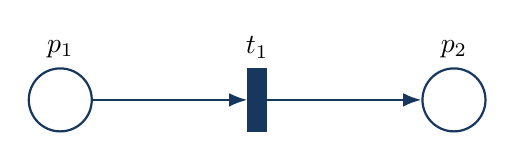
\begin{tikzpicture}
\node[pl,label=above:$p_1$] (a) at (0,0) {};
\node[tr,label=above:$t_1$] (t) at (2.5,0) {};
\node[pl,label=above:$p_2$] (b) at (5,0) {};
\draw[ar] (a)--(t);\draw[ar] (t)--(b);
\end{tikzpicture}\end{center}
\[
P=\{p_1,p_2\},\quad T=\{t_1\},\quad
A=\{(p_1,t_1),(t_1,p_2)\}.
\]
Kedua bobot arc adalah $1$.
\begin{exampleblock}{Interpretasi}
$p_1$ menyimpan pekerjaan belum diproses, $t_1$ memindahkan satu pekerjaan,
dan $p_2$ menyimpan pekerjaan yang sudah diproses.
\end{exampleblock}

\source{\S21.1, hlm. 431--434; contoh kuliah}
\end{frame}
\begin{frame}{Preset dan postset}

Untuk transisi $t$:
\[
{}^\bullet t=\{p\in P:(p,t)\in A\},\qquad
t^\bullet=\{p\in P:(t,p)\in A\}.
\]
Untuk place $p$:
\[
{}^\bullet p=\{t\in T:(t,p)\in A\},\qquad
p^\bullet=\{t\in T:(p,t)\in A\}.
\]
\begin{exampleblock}{Pada graf $p_1\to t_1\to p_2$}
\({}^\bullet t_1=\{p_1\}\) dan $t_1^\bullet=\{p_2\}$.\\
\({}^\bullet p_1=\varnothing\) dan $p_1^\bullet=\{t_1\}$.
\end{exampleblock}
Preset menunjukkan asal, postset menunjukkan tujuan.

\source{\S21.1, hlm. 431--432}
\end{frame}
\begin{frame}{Marking dan Petri net bertanda}

Marking adalah fungsi $m:P\to\N_0$ atau vektor
\[
m=(m_1,\ldots,m_n)^T\in\N_0^n,\qquad m_i=m(p_i).
\]
Sistem Petri net adalah pasangan $(N,m_0)$, dengan $m_0$ marking awal.
\begin{exampleblock}{Contoh}
Pada urutan place $(p_1,p_2)$, marking $m_0=(2,0)^T$
berarti dua token pada $p_1$ dan tidak ada token pada $p_2$.
\end{exampleblock}
Urutan place harus konsisten ketika menggunakan vektor dan matriks.

\source{\S21.1, hlm. 432}
\end{frame}
\begin{frame}{Aturan enabling}

Transisi $t_j$ \textbf{enabled} pada marking $m$ jika
\[
m_i\ge w(p_i,t_j)\quad\text{untuk setiap }p_i\in{}^\bullet t_j.
\]
Bobot dianggap $0$ untuk pasangan yang tidak memiliki arc.
\begin{exampleblock}{Contoh}
$t$ membutuhkan dua token dari $p_1$ dan satu dari $p_2$.
\[
m=(2,1)^T:\ \text{enabled},\qquad
m=(3,0)^T:\ \text{tidak enabled}.
\]
\end{exampleblock}
Token berlebih pada satu input tidak menggantikan kekurangan pada input lainnya.

\source{\S21.1, hlm. 432}
\end{frame}
\begin{frame}{Aturan firing}

Jika transisi enabled $t_j$ dipilih untuk firing, marking baru adalah
\[
m'_i=m_i-w(p_i,t_j)+w(t_j,p_i).
\]
\begin{enumerate}
\item Ambil token dari setiap input sesuai bobot arc.
\item Tambahkan token ke setiap output sesuai bobot arc.
\end{enumerate}
Notasi $m[t_j\rangle m'$ berarti firing $t_j$ membawa $m$ ke $m'$.
\begin{block}{Enabled berbeda dari sudah firing}
Pada Petri net tanpa waktu, enabling hanya menyatakan kemungkinan.
Kejadian tidak wajib berlangsung segera.
\end{block}

\source{\S21.1, hlm. 432}
\end{frame}
\begin{frame}{Contoh firing berbobot}

\begin{center}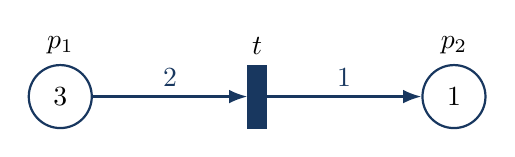
\begin{tikzpicture}
\node[pl,label=above:$p_1$] (a) at (0,0) {3};
\node[tr,label=above:$t$] (t) at (2.5,0) {};
\node[pl,label=above:$p_2$] (b) at (5,0) {1};
\draw[ar] (a)--node[above]{2}(t);
\draw[ar] (t)--node[above]{1}(b);
\end{tikzpicture}\end{center}
Angka di dalam place menyatakan banyaknya token.
\[
m=\mpmat{3\\1},\qquad m'=\mpmat{3-2\\1+1}=\mpmat{1\\2}.
\]
Firing kedua tidak dapat dilakukan karena $p_1$ tinggal memiliki satu token.
Bobot arc adalah kebutuhan token, bukan durasi.

\source{\S21.1, hlm. 431--434; contoh kuliah}
\end{frame}
\begin{frame}{Perubahan token: sebelum dan sesudah firing}

\begin{center}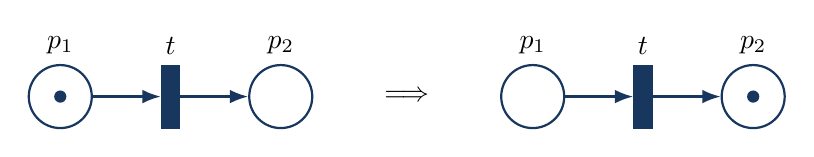
\begin{tikzpicture}
\node[pl,label=above:$p_1$] (a) at (0,0) {};\tok{a}
\node[tr,label=above:$t$] (t) at (1.4,0) {};
\node[pl,label=above:$p_2$] (b) at (2.8,0) {};
\draw[ar] (a)--(t);\draw[ar] (t)--(b);
\node at (4.4,0) {$\Longrightarrow$};
\node[pl,label=above:$p_1$] (c) at (6,0) {};
\node[tr,label=above:$t$] (v) at (7.4,0) {};
\node[pl,label=above:$p_2$] (d) at (8.8,0) {};\tok{d}
\draw[ar] (c)--(v);\draw[ar] (v)--(d);
\end{tikzpicture}\end{center}
\[
\mpmat{1\\0}[t\rangle\mpmat{0\\1}.
\]
Sesudah firing, $t$ tidak enabled karena input $p_1$ kosong.
\begin{block}{Interpretasi}
Satu kejadian mengonsumsi kondisi awal dan menghasilkan kondisi berikutnya.
\end{block}

\source{\S21.1, hlm. 431--434; contoh kuliah}
\end{frame}
\begin{frame}{Representasi matriks Pre dan Post}

Definisikan matriks berukuran $n\times m$:
\[
\Pre_{ij}=w(p_i,t_j),\quad\Post_{ij}=w(t_j,p_i),\quad C_{\rm inc}=\Post-\Pre.
\]
Kolom $j$ menyimpan kebutuhan dan produksi token oleh $t_j$.
\[
t_j\text{ enabled}\iff m\ge\Pre_{\cdot j},\qquad
m'=m+C_{{\rm inc},\cdot j}.
\]
\begin{block}{Dua jenis aljabar}
Ini aritmetika bilangan bulat biasa. Max-plus digunakan nanti untuk waktu kejadian.
$C_{\rm inc}$ berbeda dari matriks keluaran $C$ pada model dioid.
\end{block}

\source{Aturan \S21.1 ditulis dalam bentuk matriks}
\end{frame}
\begin{frame}{Contoh matriks pada rantai dua transisi}

Untuk $p_1\to t_1\to p_2\to t_2\to p_3$:
\[
\Pre=\mpmat{1&0\\0&1\\0&0},\quad\Post=\mpmat{0&0\\1&0\\0&1},\quad
C_{\rm inc}=\mpmat{-1&0\\1&-1\\0&1}.
\]
Dari $m_0=(1,0,0)^T$:
\[
m_0[t_1\rangle(0,1,0)^T[t_2\rangle(0,0,1)^T.
\]
Periksa enabling setiap kali sebelum menambahkan kolom insidensi.

\source{\S21.1, hlm. 431--434; contoh kuliah}
\end{frame}
\begin{frame}{Sinkronisasi pada Petri net}

\begin{center}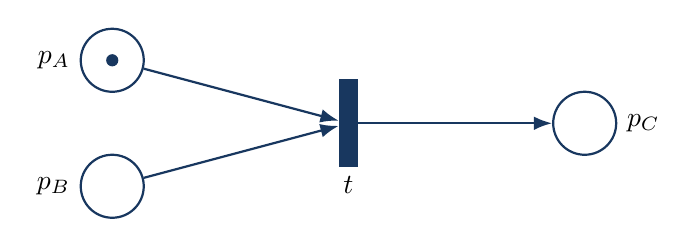
\begin{tikzpicture}
\node[pl,label=left:$p_A$] (a) at (0,.8) {};\tok{a}
\node[pl,label=left:$p_B$] (b) at (0,-.8) {};
\node[tall,label=below:$t$] (t) at (3,0) {};
\node[pl,label=right:$p_C$] (c) at (6,0) {};
\draw[ar] (a)--(t);\draw[ar] (b)--(t);\draw[ar] (t)--(c);
\end{tikzpicture}\end{center}
$t$ belum enabled karena $p_B$ kosong.
Setelah $p_B$ mendapat satu token, firing $t$ mengonsumsi satu token
dari \textbf{masing-masing} $p_A$ dan $p_B$.
\medskip

Contoh aplikasi: perakitan menunggu dua komponen.

\source{\S21.1, hlm. 431--434; contoh kuliah}
\end{frame}
\begin{frame}{Konflik: satu token, dua pilihan}

\begin{center}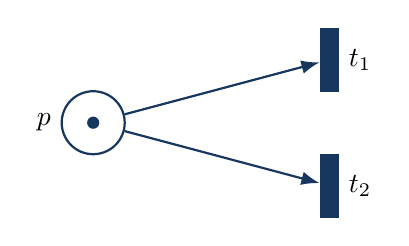
\begin{tikzpicture}
\node[pl,label=left:$p$] (p) at (0,0) {};\tok{p}
\node[tr,label=right:$t_1$] (a) at (3,.8) {};
\node[tr,label=right:$t_2$] (b) at (3,-.8) {};
\draw[ar] (p)--(a);\draw[ar] (p)--(b);
\end{tikzpicture}\end{center}
Kedua transisi enabled pada marking awal.
Jika $t_1$ firing, token habis dan $t_2$ tidak lagi enabled.
\begin{block}{Konflik berbeda dari sinkronisasi}
Pada konflik, transisi bersaing atas token yang sama.
Pada sinkronisasi, satu transisi membutuhkan token dari beberapa place.
\end{block}

\source{\S21.1, hlm. 431--434; contoh kuliah}
\end{frame}
\begin{frame}{Konkurensi: dua kejadian independen}

\begin{center}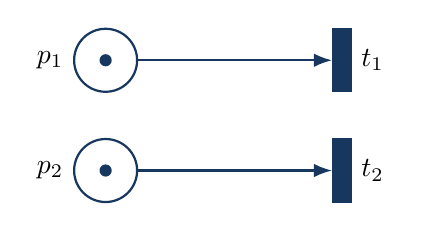
\begin{tikzpicture}
\node[pl,label=left:$p_1$] (a) at (0,.7) {};\tok{a}
\node[tr,label=right:$t_1$] (b) at (3,.7) {};
\node[pl,label=left:$p_2$] (c) at (0,-.7) {};\tok{c}
\node[tr,label=right:$t_2$] (d) at (3,-.7) {};
\draw[ar] (a)--(b);\draw[ar] (c)--(d);
\end{tikzpicture}\end{center}
$t_1$ dan $t_2$ menggunakan place berbeda.
Firing salah satunya tidak menghilangkan enabling yang lain.
\[
m[t_1t_2\rangle m'\qquad\text{dan}\qquad m[t_2t_1\rangle m'.
\]
Pada contoh ini, kedua urutan menghasilkan marking akhir sama.

\source{\S21.1, hlm. 431--434; contoh kuliah}
\end{frame}
\begin{frame}{Self-loop pada sebuah place}

\begin{center}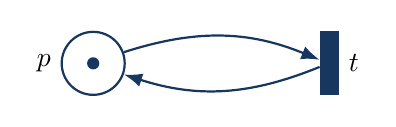
\begin{tikzpicture}
\node[pl,label=left:$p$] (p) at (0,0) {};\tok{p}
\node[tr,label=right:$t$] (t) at (3,0) {};
\draw[ar] (p) to[bend left=20] (t);
\draw[ar] (t) to[bend left=20] (p);
\end{tikzpicture}\end{center}
Dengan bobot $1$, $m'(p)=m(p)-1+1=m(p)$.
Meskipun token bersih tidak berubah, $t$ tetap membutuhkan token di $p$.
\begin{block}{Makna}
Kolom insidensi nol tidak berarti transisi selalu enabled.
Syarat enabling tetap dibaca dari $\Pre$.
\end{block}

\source{\S21.1, hlm. 431--434; contoh kuliah}
\end{frame}
\begin{frame}{Sifat perilaku Petri net}

\begin{description}
\item[Terjangkau] Marking diperoleh dari $m_0$ melalui urutan firing yang sah.
\item[Deadlock] Tidak ada transisi enabled pada marking tersebut.
\item[Bounded] Jumlah token setiap place dibatasi suatu bilangan hingga pada semua marking terjangkau.
\item[Live] Dari setiap marking terjangkau, setiap transisi dapat firing setelah suatu kelanjutan yang sesuai.
\end{description}
\begin{block}{Pemeriksaan}
Marking dengan token tidak selalu bebas deadlock.
Boundedness tidak dengan sendirinya menjamin liveness.
\end{block}

\source{Definisi dasar untuk melengkapi \S21.1}
\end{frame}
\begin{frame}{Siklus tanpa token dan deadlock}

\begin{center}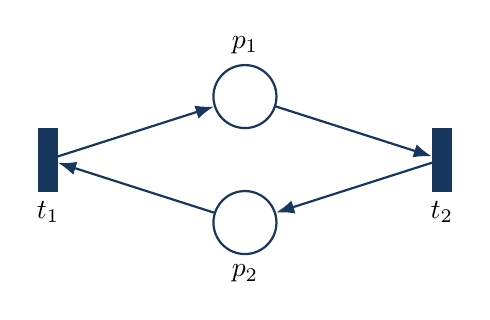
\begin{tikzpicture}
\node[tr,label=below:$t_1$] (a) at (0,0) {};
\node[tr,label=below:$t_2$] (b) at (5,0) {};
\node[pl,label=above:$p_1$] (p) at (2.5,.8) {};
\node[pl,label=below:$p_2$] (q) at (2.5,-.8) {};
\draw[ar] (a)--(p);\draw[ar] (p)--(b);
\draw[ar] (b)--(q);\draw[ar] (q)--(a);
\end{tikzpicture}\end{center}
Jika $m_0=(0,0)^T$, kedua transisi menunggu token.
Dengan satu token pada $p_2$, urutan $t_1,t_2,t_1,t_2,\ldots$ dimungkinkan.
\medskip

Struktur graf saja belum menentukan perilaku. Marking awal juga penting.

\source{\S21.1, hlm. 431--434; contoh kuliah}
\end{frame}
\begin{frame}{Latihan: membaca dan menjalankan Petri net}

Untuk rantai $p_1\to t_1\to p_2\to t_2\to p_3$,
semua bobot $1$, dan $m_0=(2,0,0)^T$:
\begin{enumerate}
\item Transisi mana yang enabled pada awal?
\item Tentukan marking setelah urutan $t_1,t_2,t_1$.
\item Apakah urutan $t_2,t_1$ sah dari $m_0$?
\item Berapa jumlah total token pada setiap marking terjangkau?
\end{enumerate}
\begin{block}{Petunjuk}
Periksa enabling sebelum memperbarui marking.
\end{block}

\end{frame}
\begin{frame}{Pembahasan: urutan firing dan invariant}

Pada awal, hanya $t_1$ enabled.
\[
(2,0,0)^T\xrightarrow{t_1}(1,1,0)^T
\xrightarrow{t_2}(1,0,1)^T
\xrightarrow{t_1}(0,1,1)^T.
\]
Urutan $t_2,t_1$ tidak sah karena $t_2$ tidak enabled pada $m_0$.
\[
m_1+m_2+m_3=2
\]
pada setiap marking terjangkau.
\begin{block}{Mengapa jumlah token tetap?}
Setiap firing mengurangi dan menambahkan satu token.
Pada contoh ini, $(1,1,1)C_{\rm inc}=0$.
\end{block}
Ini contoh invariant, bukan sifat semua Petri net.

\end{frame}
\begin{frame}{Event graph dan waktu}
\begin{center}{\LARGE\bfseries\color{AcademicBlue}Event graph dan waktu}\\[8mm]Dari aturan token ke waktu kejadian\end{center}
\end{frame}
\begin{frame}{Event graph sebagai kelas khusus Petri net}

Sistem Petri net $(N,m_0)$ disebut \textbf{event graph} jika
\[
|{}^\bullet p|=|p^\bullet|=1\quad\text{untuk setiap }p\in P
\]
dan bobot semua arc adalah $1$.
\begin{itemize}
\item Setiap place memiliki satu produsen dan satu konsumen token.
\item Transisi boleh memiliki beberapa input atau output place.
\item Sinkronisasi tetap dapat terjadi.
\item Konflik pemilihan konsumen token tidak terjadi.
\end{itemize}
Event graph juga disebut \textit{synchronization graph}.

\source{\S21.1, hlm. 433}
\end{frame}
\begin{frame}{Contoh event graph yang lengkap}

\begin{center}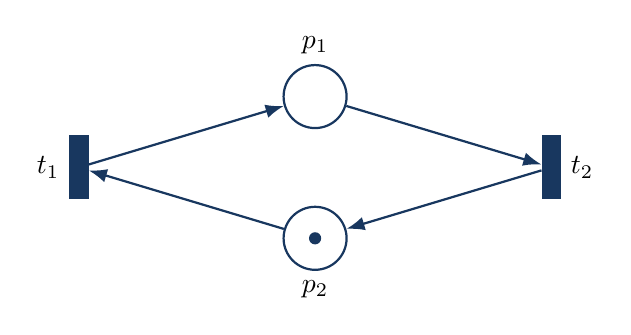
\begin{tikzpicture}
\node[tr,label=left:$t_1$] (a) at (0,0) {};
\node[tr,label=right:$t_2$] (b) at (6,0) {};
\node[pl,label=above:$p_1$] (p) at (3,.9) {};
\node[pl,label=below:$p_2$] (q) at (3,-.9) {};\tok{q}
\draw[ar] (a)--(p);\draw[ar] (p)--(b);
\draw[ar] (b)--(q);\draw[ar] (q)--(a);
\end{tikzpicture}\end{center}
Pada $p_1$: produsen $t_1$, konsumen $t_2$.
Pada $p_2$: produsen $t_2$, konsumen $t_1$.
\medskip

Semua place memenuhi syarat event graph.
Satu token awal memungkinkan kejadian bergantian.

\source{\S21.1, hlm. 431--434; contoh kuliah}
\end{frame}
\begin{frame}{Contoh yang bukan event graph}

\begin{center}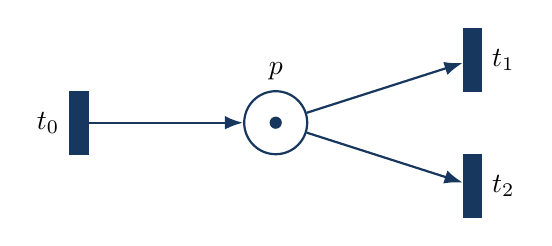
\begin{tikzpicture}
\node[tr,label=left:$t_0$] (a) at (0,0) {};
\node[pl,label=above:$p$] (p) at (2.5,0) {};\tok{p}
\node[tr,label=right:$t_1$] (b) at (5,.8) {};
\node[tr,label=right:$t_2$] (c) at (5,-.8) {};
\draw[ar] (a)--(p);\draw[ar] (p)--(b);\draw[ar] (p)--(c);
\end{tikzpicture}\end{center}
Place $p$ mempunyai dua transisi keluaran:
\[
p^\bullet=\{t_1,t_2\},\qquad |p^\bullet|=2.
\]
Struktur ini mengandung pilihan atau konflik dan melanggar syarat event graph.

\source{\S21.1, hlm. 431--434; contoh kuliah}
\end{frame}
\begin{frame}{Petri net dengan waktu}

Petri net tanpa waktu menentukan \textbf{urutan kejadian yang mungkin}.
Informasi waktu diperlukan untuk menentukan kapan kejadian berlangsung.
\begin{itemize}
\item Waktu pada transisi: delay yang dikaitkan dengan firing.
\item Waktu pada place: holding time token sebelum boleh digunakan.
\end{itemize}
\begin{block}{Konvensi materi selanjutnya}
TEG diberi holding time deterministik pada place.
Untuk analisis paling awal, transisi firing segera setelah seluruh input siap.
\end{block}
Banyak variasi timed Petri net tersedia. Semantik waktu harus dinyatakan,
terutama jika model memuat konflik atau kapasitas layanan.

\source{\S21.1, hlm. 433--434; \S16.2.2}
\end{frame}
\begin{frame}{Timed Petri net dan time Petri net}

Menurut klasifikasi buku:
\begin{center}\begin{tabular}{lll}\toprule
Jenis&Waktu&Contoh pada transisi\\\midrule
Timed Petri net&Satu nilai $\theta$&Delay deterministik $\theta$\\
Time Petri net&Interval $[\ell,u]$&Firing di antara batas waktu\\\bottomrule
\end{tabular}\end{center}
Jika enabled pada $\tau$ dan tetap enabled:
\begin{itemize}
\item Pada contoh T-timed: firing pada $\tau+\theta$.
\item Pada contoh T-time: tidak sebelum $\tau+\ell$ dan tidak sesudah $\tau+u$.
\end{itemize}
Awalan T menyatakan waktu pada transisi. Awalan P menyatakan waktu pada place.
Materi dioid berfokus pada TEG dengan holding time tetap.

\source{\S16.2.2, hlm. 321; \S21.1, hlm. 433}
\end{frame}
\begin{frame}{Holding time dan token yang belum siap}

Misalkan token masuk ke place $p$ pada waktu $2$, dengan holding time $h=3$.
\[
t_{\rm siap}=2+3=5.
\]
\begin{center}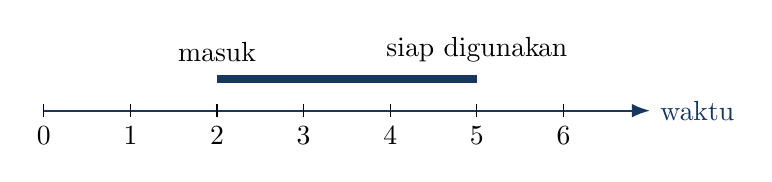
\begin{tikzpicture}[x=1.1cm]
\draw[ar] (0,0)--(7,0) node[right]{waktu};
\foreach \x in {0,1,2,3,4,5,6}
 {\draw (\x,.08)--(\x,-.08) node[below] {$\x$};}
\draw[line width=3pt,AcademicBlue] (2,.4)--(5,.4);
\node[above] at (2,.5) {masuk};
\node[above] at (5,.5) {siap digunakan};
\end{tikzpicture}\end{center}
Token sudah ada pada waktu $3$, tetapi belum dapat digunakan.
\begin{block}{Dua jenis kesiapan}
Jumlah token memenuhi syarat struktural belum tentu berarti syarat waktunya terpenuhi.
\end{block}

\source{\S21.1, hlm. 431--434; contoh kuliah}
\end{frame}
\begin{frame}{Timed event graph}

Timed event graph (TEG) adalah event graph yang dilengkapi informasi waktu.
Dalam materi ini:
\[
\mathcal G=(N,m_0,h),\qquad h:P\to\mathbb R_{\ge0}.
\]
\begin{itemize}
\item $N$: graf event graph berbobot unit.
\item $m_0$: jumlah token awal.
\item $h(p)$: holding time token pada $p$.
\end{itemize}
Untuk token awal, tentukan pula waktu ketersediaannya atau riwayat yang ekuivalen.
\begin{block}{Pemisahan konsep}
Struktur mengatur ketergantungan. Token awal mengatur offset kejadian.
Holding time mengatur durasi.
\end{block}

\source{\S21.1, hlm. 433--434}
\end{frame}
\begin{frame}{Empat kelas model yang sudah diperkenalkan}

\begin{center}\begin{tabular}{p{2.6cm}p{5cm}p{4cm}}\toprule
Model&Struktur&Waktu\\\midrule
Petri net&Graf bipartit, marking, firing&Tidak ditentukan\\[2mm]
Event graph&Setiap place: satu input, satu output; bobot 1&Tidak ditentukan\\[2mm]
Timed Petri net&Petri net dengan semantik delay&Delay pada place atau transisi\\[2mm]
Timed event graph&Event graph dengan semantik waktu&Di sini: holding time pada place\\\bottomrule
\end{tabular}\end{center}
Syarat event graph membatasi struktur. Penambahan waktu memperkaya semantik.

\source{\S21.1; \S16.2.2}
\end{frame}
\begin{frame}{Memindahkan delay transisi pada TEG}

Delay deterministik suatu transisi dapat dipindahkan ke seluruh
place masukannya pada representasi TEG yang digunakan buku.
\begin{exampleblock}{Persamaan penjelas}
Jika waktu mulai paling awal $s=\max(a,b)$ dan delay transisi $d$,
waktu selesai adalah
\[
y=s+d=\max(a+d,b+d).
\]
\end{exampleblock}
Karena itu, delay $d$ dapat dipandang sebagai tambahan pada kedua jalur masuk.
\medskip\textbf{Batas pernyataan.}
Kesetaraan ini berkaitan dengan representasi waktu kejadian TEG.
Semantik timed Petri net umum dapat berbeda.

\source{\S21.1, hlm. 433}
\end{frame}
\begin{frame}{Dater: waktu firing ke-k}

Tuliskan $x_j(k)$ untuk waktu firing ke-$k$ dari transisi $t_j$.
Karena kejadian diurutkan:
\[
x_j(k+1)\ge x_j(k).
\]
Beberapa kejadian dapat mempunyai waktu sama jika model mengizinkannya.
\begin{exampleblock}{Contoh}
\[
x_j(1)=2,\quad x_j(2)=5,\quad x_j(3)=5.
\]
Kejadian kedua dan ketiga berlangsung pada waktu yang sama.
\end{exampleblock}
Indeks kejadian $k$ dan waktu fisik $t$ adalah besaran berbeda.

\source{\S21.1 dan \S21.4}
\end{frame}
\begin{frame}{Ilustrasi TEG: satu ketergantungan}


\begin{center}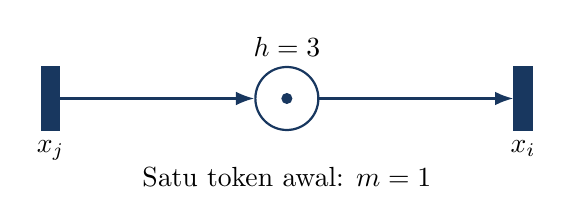
\begin{tikzpicture}
\node[tr,label=below:$x_j$] (a) at (0,0) {};
\node[pl,label={above:$h=3$}] (p) at (3,0) {};
\node[tr,label=below:$x_i$] (b) at (6,0) {};
\fill[AcademicBlue] (p.center) circle (2pt);
\draw[ar] (a)--(p);\draw[ar] (p)--(b);
\node at (3,-1) {Satu token awal: $m=1$};
\end{tikzpicture}\end{center}
Jika $x_j(k)$ adalah waktu kejadian ke-$k$, ketergantungannya:
\[
x_i(k)\ge x_j(k-1)+3.
\]
Untuk perilaku paling awal dengan hanya ketergantungan ini, berlaku persamaan.
Token awal harus memiliki waktu ketersediaan yang ditentukan.

\source{\S21.1, hlm. 433--434; ilustrasi kuliah}

\end{frame}
\begin{frame}{Mengapa token awal menggeser indeks?}

Place $p$ menerima token dari $t_r$ dan mempunyai $m_0(p)$ token awal.
Token baru dari firing ke-$k$ transisi $t_r$ merupakan token ke-$(k+m_0(p))$ di $p$.
\[
\pi_p(k+m_0(p))=x_r(k).
\]
Setelah holding time $h_p$:
\[
x_j(k)\ge x_r(k-m_0(p))+h_p.
\]
\begin{exampleblock}{Contoh}
$m_0(p)=2$ dan $h_p=4$ memberi
$x_j(k)\ge x_r(k-2)+4$.
\end{exampleblock}
Untuk firing awal yang memakai token awal, diperlukan data kesiapan token tersebut.

\source{\S21.1, hlm. 434}
\end{frame}
\begin{frame}{Penurunan persamaan waktu paling awal}

Untuk setiap place input $p$ dari $t_j$:
\[
x_j(k)\ge\pi_p(k)+h_p.
\]
Semua kendala harus terpenuhi. Maka waktu paling awalnya:
\[
x_j(k)=\max_{p\in{}^\bullet t_j}\{\pi_p(k)+h_p\}.
\]
Jika $t_r$ adalah transisi produsen token pada $p$:
\[
\pi_p(k)=x_r(k-m_0(p)).
\]
Dengan substitusi, persamaan TEG hanya memuat dater transisi.

\source{\S21.1, hlm. 434}
\end{frame}
\begin{frame}{Sinkronisasi beberapa prasyarat}


Untuk dua prasyarat dengan waktu siap $x_1(k)+2$ dan $x_2(k-1)+5$:
\[
y(k)\ge x_1(k)+2,\qquad y(k)\ge x_2(k-1)+5.
\]
Waktu paling awal yang memenuhi keduanya adalah
\[
y(k)=\max\{x_1(k)+2,\ x_2(k-1)+5\}.
\]
\begin{exampleblock}{Contoh}
Jika $x_1(k)=6$ dan $x_2(k-1)=4$, maka $y(k)=\max(8,9)=9$.
\end{exampleblock}
Persamaan paling awal mengasumsikan transisi berlangsung segera setelah seluruh prasyarat terpenuhi.

\source{\S21.1; contoh numerik kuliah}

\end{frame}
\begin{frame}{Contoh sinkronisasi bertempo}

Dua token masuk ke input place suatu transisi pada waktu $1$ dan $4$.
Holding time kedua place adalah $3$ dan $2$.
\[
r_1=1+3=4,\qquad r_2=4+2=6.
\]
\[
x_{\rm awal}=\max(r_1,r_2)=6.
\]
\begin{center}\begin{tabular}{lrrr}\toprule
Input&Masuk&Holding time&Siap\\\midrule
1&1&3&4\\
2&4&2&6\\\bottomrule
\end{tabular}\end{center}
Firing pada $5$ melanggar input kedua. Firing pada $8$ mungkin memenuhi batas
minimum, tetapi bukan perilaku paling awal.

\source{\S21.1, hlm. 431--434; contoh kuliah}
\end{frame}
\begin{frame}{Latihan: struktur, token, atau waktu?}

\begin{enumerate}
\item Place memiliki dua output transition. Apakah ini event graph?
\item Arc berbobot $2$. Apakah ini event graph menurut definisi buku?
\item Satu token masuk pada waktu $3$ dan holding time $4$.
Kapan token siap?
\item Place dengan dua token awal dan holding time $5$
menghubungkan $x_1$ ke $x_2$. Tuliskan kendala dater.
\end{enumerate}

\end{frame}
\begin{frame}{Pembahasan: struktur, token, dan waktu}

\begin{enumerate}
\item Bukan event graph karena $|p^\bullet|=2$.
\item Bukan event graph karena semua bobot harus $1$.
\item Token siap pada $3+4=7$.
\item Untuk bagian yang ditentukan riwayat produsen:
\[
x_2(k)\ge x_1(k-2)+5.
\]
Jika ini satu-satunya prasyarat dan berlaku semantik paling awal,
gunakan persamaan.
\end{enumerate}
Jumlah token awal berbeda dari bobot arc.
Dua token pada place tetap diperbolehkan pada event graph.

\end{frame}
\begin{frame}{Dioid dan max-plus}
\begin{center}{\LARGE\bfseries\color{AcademicBlue}Dioid dan max-plus}\\[8mm]Aljabar untuk sinkronisasi dan keterlambatan\end{center}
\end{frame}
\begin{frame}{Operasi biner dan monoid}

Operasi biner pada $D$ adalah fungsi $D\times D\to D$.
Struktur $(D,\circ,e)$ adalah \textbf{monoid} jika
\[
(a\circ b)\circ c=a\circ(b\circ c),\qquad
e\circ a=a\circ e=a.
\]
Jika $a\circ b=b\circ a$, monoid tersebut komutatif.
\begin{exampleblock}{Contoh}
$(\mathbb Z,+,0)$ adalah monoid komutatif.
$(\mathbb R,\max,-\infty)$ menjadi monoid setelah $-\infty$ ditambahkan ke himpunannya.
\end{exampleblock}
Invers tidak disyaratkan. Contohnya, pada maksimum tidak ada operasi
yang mengembalikan bilangan hingga ke identitas $-\infty$.

\source{\S21.3, hlm. 437}
\end{frame}
\begin{frame}{Dioid: semiring dengan penjumlahan idempoten}


Dioid $(D,\oplus,\otimes,\eps,e)$ memenuhi:
\begin{enumerate}
\item $(D,\oplus,\eps)$ monoid komutatif dan $a\oplus a=a$;
\item $(D,\otimes,e)$ monoid;
\item perkalian distributif terhadap penjumlahan;
\item $\eps\otimes a=a\otimes\eps=\eps$.
\end{enumerate}
\begin{block}{Notasi}
$\eps$ adalah identitas penjumlahan, sedangkan $e$ adalah identitas perkalian.
Keduanya tidak harus berupa bilangan $0$ dan $1$.
\end{block}
Monoid berarti operasi tertutup, asosiatif, dan memiliki elemen identitas.

\source{\S21.3, hlm. 437}

\end{frame}
\begin{frame}{Max-plus dan min-plus}


\begin{center}\begin{tabular}{lcc}\toprule
&Max-plus&Min-plus\\\midrule
Himpunan dasar&$\mathbb Z\cup\{-\infty\}$&$\mathbb Z\cup\{+\infty\}$\\
$a\oplus b$&$\max(a,b)$&$\min(a,b)$\\
$a\otimes b$&$a+b$&$a+b$\\
$\eps$&$-\infty$&$+\infty$\\
$e$&$0$&$0$\\\bottomrule
\end{tabular}\end{center}
Contoh max-plus: $3\oplus5=5$, $3\otimes5=8$.
\medskip

Versi lengkap menambahkan elemen tak hingga lainnya dengan konvensi
$\eps$ tetap menyerap pada perkalian.
Dalam contoh hitungan, bilangan hingga cukup digunakan.

\source{\S21.3, hlm. 437--438}

\end{frame}
\begin{frame}{Mengapa operasi max-plus memenuhi aksioma?}


\begin{align*}
a\oplus a&=\max(a,a)=a,\\
a\oplus\eps&=\max(a,-\infty)=a,\\
a\otimes e&=a+0=a.
\end{align*}
Untuk $a,b,c$ hingga:
\[
a+\max(b,c)=\max(a+b,a+c).
\]
Ini adalah distributivitas $\otimes$ terhadap $\oplus$.
\begin{block}{Perbedaan dengan lapangan}
Tidak ada invers penjumlahan untuk elemen hingga:
$\max(a,b)$ tidak mungkin bernilai $-\infty$ jika $a$ hingga.
\end{block}

\source{\S21.3; penjabaran kuliah}

\end{frame}
\begin{frame}{Pangkat dan pembatalan dalam max-plus}

Untuk $a$ hingga dan bilangan bulat $r\ge1$:
\[
a^r=\underbrace{a\otimes\cdots\otimes a}_{r\text{ kali}}=ra
\]
pada aritmetika biasa. Contoh: $3^2=3\otimes3=6$ dalam max-plus.
\begin{block}{Penjumlahan tidak dapat dibatalkan}
\[
2\oplus5=3\oplus5=5,\qquad 2\ne3.
\]
Dari $a\oplus c=b\oplus c$ tidak dapat disimpulkan $a=b$.
\end{block}
Hindari menggunakan aturan pengurangan aljabar biasa untuk menghilangkan suku $\oplus$.

\source{\S21.3--21.4, hlm. 437--440}
\end{frame}
\begin{frame}{Urutan alami suatu dioid}


Definisi:
\[
a\preceq b\quad\Longleftrightarrow\quad a\oplus b=b.
\]
\begin{itemize}
\item Di max-plus: $a\preceq b$ sama dengan $a\le b$ biasa.
\item Di min-plus: $a\preceq b$ sama dengan $a\ge b$ biasa.
\end{itemize}
\begin{exampleblock}{Contoh}
Max-plus: $3\oplus5=5$, sehingga $3\preceq5$.\\
Min-plus: $5\oplus3=3$, sehingga $5\preceq3$.
\end{exampleblock}
Simbol $\preceq$ selalu merujuk urutan dioid yang sedang digunakan.

\source{\S21.3, hlm. 437}

\end{frame}
\begin{frame}{Mengapa urutan alami merupakan urutan parsial?}

Definisikan $a\preceq b\iff a\oplus b=b$.
\begin{description}
\item[Refleksif] $a\oplus a=a$ karena idempotensi.
\item[Antisimetris] Jika $a\oplus b=b$ dan $b\oplus a=a$,
komutativitas memberi $a=b$.
\item[Transitif] Jika $a\oplus b=b$ dan $b\oplus c=c$, maka
\[
a\oplus c=a\oplus(b\oplus c)
=(a\oplus b)\oplus c=b\oplus c=c.
\]
\end{description}
Pada max-plus, urutannya total. Pada dioid deret,
dua elemen dapat tidak dapat dibandingkan.

\source{\S21.3, hlm. 437; bukti dijabarkan}
\end{frame}
\begin{frame}{Supremum, infimum, dan kelengkapan}

Dalam urutan $\preceq$:
\begin{itemize}
\item $a\oplus b$ adalah supremum: batas atas terkecil dari $a,b$.
\item $a\wedge b$ adalah infimum jika batas bawah terbesar itu ada.
\item Dioid lengkap memiliki semua supremum, termasuk jumlah tak hingga.
\end{itemize}
Pada max-plus lengkap:
\[
a\oplus b=\max(a,b),\qquad a\wedge b=\min(a,b).
\]
Pada min-plus lengkap, urutan berbalik:
\[
a\oplus b=\min(a,b),\qquad a\wedge b=\max(a,b).
\]
Jadi simbol $\wedge$ harus dibaca menurut urutan dioidnya.

\source{\S21.3, hlm. 437}
\end{frame}
\begin{frame}{Monotonisitas operasi dioid}

Jika $a\preceq b$, maka
\[
a\oplus c\preceq b\oplus c,\qquad
ca\preceq cb,\qquad ac\preceq bc.
\]
Contoh pembuktian untuk perkalian kiri:
\[
a\oplus b=b
\ \Longrightarrow\
ca\oplus cb=c(a\oplus b)=cb.
\]
\begin{block}{Arti untuk sistem bertempo}
Jika waktu masukan ditunda, model max-plus yang sama tidak menghasilkan
waktu keluaran yang lebih awal.
\end{block}
Monotonisitas menjadi dasar iterasi solusi dan teori residuasi.

\source{\S22.2.1; konsekuensi aksioma dioid}
\end{frame}
\begin{frame}{Matriks di atas dioid}


Operasi matriks menggunakan pola yang sama dengan aljabar biasa:
\[
(A\oplus B)_{ij}=A_{ij}\oplus B_{ij},\qquad
(A\otimes B)_{ij}=\bigoplus_k A_{ik}\otimes B_{kj}.
\]
Pada max-plus:
\[
(A\otimes B)_{ij}=\max_k(A_{ik}+B_{kj}).
\]
Matriks identitas dioid:
\[
E=\mpmat{e&\eps\\\eps&e}
=\mpmat{0&-\infty\\-\infty&0}.
\]
Elemen $0$ hingga menyatakan durasi nol. $\eps$ menyatakan tidak ada kontribusi.

\source{\S21.3, hlm. 438}

\end{frame}
\begin{frame}{Contoh perkalian matriks max-plus}


Gunakan matriks jaringan transportasi pada buku:
\[
A=\mpmat{2&5\\3&3},\qquad x=\mpmat{0\\0}.
\]
\[
A\otimes x=
\mpmat{\max(2+0,5+0)\\\max(3+0,3+0)}
=\mpmat{5\\3}.
\]
Perkalian kedua:
\[
A\otimes\mpmat{5\\3}
=\mpmat{\max(7,8)\\\max(8,6)}
=\mpmat{8\\8}.
\]

\source{\S21.2--21.4, hlm. 435--438}

\end{frame}
\begin{frame}{Representasi graf sebuah matriks max-plus}

Untuk matriks $A$, simpul $j$ memiliki arc menuju simpul $i$
dengan bobot $A_{ij}$ jika $A_{ij}\ne\eps$.
\begin{exampleblock}{Contoh}
Matriks $A=\mpmat{2&5\\3&3}$ memiliki loop berbobot $2$ pada simpul 1, loop berbobot $3$ pada simpul 2,
arc $1\to2$ berbobot $3$, dan arc $2\to1$ berbobot $5$.
\end{exampleblock}
\[
(A^2)_{ij}=\max_\ell(A_{i\ell}+A_{\ell j})
\]
adalah bobot maksimum lintasan dua arc dari $j$ ke $i$.
Panjang lintasan dihitung dari banyak arc, bukan total bobot.

\source{\S21.3--21.4, hlm. 437--440}
\end{frame}
\begin{frame}{TEG jaringan transportasi dari buku}

\begin{center}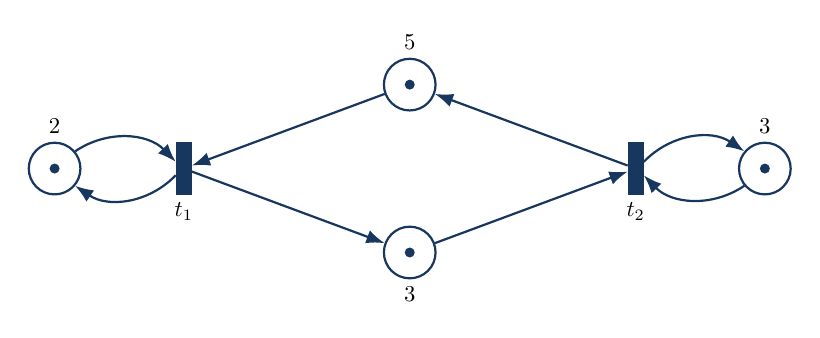
\begin{tikzpicture}[scale=.82,transform shape]
\node[tr,label=below:$t_1$] (a) at (0,0) {};
\node[tr,label=below:$t_2$] (b) at (7,0) {};
\node[pl,label=above:$5$] (p) at (3.5,1.3) {};\tok{p}
\node[pl,label=below:$3$] (q) at (3.5,-1.3) {};\tok{q}
\node[pl,label=above:$2$] (l) at (-2,0) {};\tok{l}
\node[pl,label=above:$3$] (r) at (9,0) {};\tok{r}
\draw[ar] (b)--(p);\draw[ar] (p)--(a);
\draw[ar] (a)--(q);\draw[ar] (q)--(b);
\draw[ar] (a) to[bend left=40] (l);
\draw[ar] (l) to[bend left=40] (a);
\draw[ar] (b) to[bend left=40] (r);
\draw[ar] (r) to[bend left=40] (b);
\end{tikzpicture}\end{center}
Titik menyatakan kereta. Angka di luar place menyatakan waktu perjalanan.
Firing $t_1,t_2$ menyatakan keberangkatan di kedua stasiun.

\source{\S21.2, Gambar 21.4, hlm. 435; digambar ulang}
\end{frame}
\begin{frame}{Jaringan transportasi: arti persamaannya}


Pada dua stasiun, keberangkatan menunggu kedatangan kereta terkait.
\begin{align*}
x_1(k+1)&=\max\{x_1(k)+2,\ x_2(k)+5\},\\
x_2(k+1)&=\max\{x_1(k)+3,\ x_2(k)+3\}.
\end{align*}
\[
x(k+1)=A\otimes x(k),\qquad A=\mpmat{2&5\\3&3}.
\]
Variabel $x_i(k)$ menyatakan waktu keberangkatan ke-$k$ di stasiun $i$.
\begin{block}{Linier dalam aljabar yang dipilih}
Persamaan menggunakan maksimum dalam aljabar biasa, tetapi berbentuk linier terhadap operasi max-plus.
\end{block}

\source{\S21.2, hlm. 434--436; \S21.4}

\end{frame}
\begin{frame}{Evolusi jadwal: dua pilihan keadaan awal}


\begin{center}\begin{tabular}{c|rrrrr}\toprule
$k$&1&2&3&4&5\\\midrule
$x_1(k)$, awal $(0,0)^T$&0&5&8&13&16\\
$x_2(k)$, awal $(0,0)^T$&0&3&8&11&16\\\midrule
$x_1(k)$, awal $(1,0)^T$&1&5&9&13&17\\
$x_2(k)$, awal $(1,0)^T$&0&4&8&12&16\\\bottomrule
\end{tabular}\end{center}
Awal $(1,0)^T$ menghasilkan interval tetap $4$ pada setiap stasiun.
Awal $(0,0)^T$ menghasilkan pola interval yang bergantian.
\begin{exampleblock}{Diskusi}
Keadaan awal memengaruhi pola jadwal, walaupun matriks sistemnya sama.
\end{exampleblock}

\source{\S21.2, hlm. 435--436}

\end{frame}
\begin{frame}{Nilai eigen max-plus dan interval keberangkatan}


Pasangan eigen memenuhi $A\otimes\xi=\lambda\otimes\xi$.
Untuk
\[
A=\mpmat{2&5\\3&3},\qquad \xi=\mpmat{1\\0},\qquad\lambda=4:
\]
\[
A\otimes\xi=\mpmat{5\\4}
=\mpmat{4+1\\4+0}=\lambda\otimes\xi.
\]
Jika $x(1)=\xi$, maka
\[
x_i(k)=\xi_i+(k-1)\lambda
\]
dalam aritmetika biasa. Interval kejadian adalah $\lambda=4$ satuan waktu.

\source{\S21.4, hlm. 439--440}

\end{frame}
\begin{frame}{Siklus dan nilai eigen pada contoh}


Untuk graf max-plus yang strongly connected, nilai eigen adalah
maksimum rata-rata bobot siklus.
\begin{center}\begin{tabular}{lcc}\toprule
Siklus&Bobot total/Panjang&Rata-rata\\\midrule
$1\to1$&$2/1$&2\\
$2\to2$&$3/1$&3\\
$1\to2\to1$&$(3+5)/2$&4\\\bottomrule
\end{tabular}\end{center}
\[
\lambda=\max(2,3,4)=4.
\]
Pada graf matriks, arc $j\to i$ berbobot $A_{ij}$.
Hasil ini konsisten dengan contoh eigen pada slide sebelumnya.

\source{\S21.4, hlm. 439--440; interpretasi graf}

\end{frame}
\begin{frame}{Mengapa keadaan awal eigen menghasilkan jadwal tetap?}

Jika $A\xi=\lambda\xi$ dalam max-plus dan $x(1)=\xi$, maka
\[
x(2)=A\xi=\lambda\xi,\qquad
x(3)=A(\lambda\xi)=\lambda(A\xi)=\lambda^2\xi.
\]
Secara induksi,
\[
x(k)=\lambda^{k-1}\xi.
\]
Dalam aritmetika biasa:
\[
x_i(k)=\xi_i+(k-1)\lambda.
\]
Setiap komponen maju sebesar $\lambda$ pada setiap kejadian.
\begin{block}{Satuan}
$\lambda$ adalah waktu per kejadian. Jika $\lambda>0$, laju kejadian adalah $1/\lambda$.
\end{block}

\source{\S21.4, hlm. 439--440}
\end{frame}
\begin{frame}{Tambahan token dan perubahan kapasitas}

Buku menambahkan kereta pada jalur dari stasiun 1 ke 2.
Ketergantungan satu langkah berubah menjadi dua langkah:
\[
x_2(k+2)=\max\{x_1(k)+3,x_2(k+1)+3\}.
\]
Dengan variabel tambahan $x_3(k+1)=x_1(k)$:
\[
\mpmat{x_1(k+1)\\x_2(k+1)\\x_3(k+1)}
=
\mpmat{2&5&\eps\\\eps&3&3\\0&\eps&\eps}
\otimes\mpmat{x_1(k)\\x_2(k)\\x_3(k)}.
\]
Penambahan sumber daya mengubah offset indeks.
Model orde satu diperoleh dengan menambah variabel keadaan.

\source{\S21.2, pers. (21.11)--(21.15), hlm. 436}
\end{frame}
\begin{frame}{Jadwal setelah penambahan kereta}

Dengan awal $(0,0,0)^T$:
\begin{center}\begin{tabular}{c|rrrrr}\toprule
$k$&1&2&3&4&5\\\midrule
$x_1$&0&5&8&11&14\\
$x_2$&0&3&6&9&12\\
$x_3$&0&0&5&8&11\\\bottomrule
\end{tabular}\end{center}
Setelah transien, interval keberangkatan menjadi $3$.
Loop luar pada stasiun 2 memiliki waktu perjalanan $3$ dan satu kereta,
sehingga menjadi bottleneck berikutnya.
\begin{block}{Pertanyaan pemodelan}
Bisakah offset dua kejadian disimpan langsung,
tanpa menambah variabel $x_3$? Inilah motivasi operator $\gamma$.
\end{block}

\source{\S21.2, hlm. 436; \S21.5}
\end{frame}
\begin{frame}{Latihan: operasi matriks dan pasangan eigen}


Gunakan max-plus dan
\[
A=\mpmat{1&4\\2&2},\qquad x(1)=\mpmat{0\\0}.
\]
\begin{enumerate}
\item Hitung $x(2)$ dan $x(3)$.
\item Hitung $A^2=A\otimes A$.
\item Periksa apakah $\lambda=3$ dan $\xi=(1,0)^T$ merupakan pasangan eigen.
\item Jelaskan arti $\eps$ dan $e$ pada matriks max-plus.
\end{enumerate}
 


\end{frame}
\begin{frame}{Pembahasan: operasi matriks dan pasangan eigen}


\[
x(2)=\mpmat{4\\2},\qquad
x(3)=\mpmat{6\\6}.
\]
\[
A^2=\mpmat{\max(2,6)&\max(5,6)\\
\max(3,4)&\max(6,4)}
=\mpmat{6&6\\4&6}.
\]
\[
A\otimes\mpmat{1\\0}=\mpmat{4\\3}
=3\otimes\mpmat{1\\0}.
\]
Jadi pasangan eigen benar. Pada max-plus, $\eps=-\infty$ dan $e=0$.


\end{frame}
\begin{frame}{Satuan waktu dan eksponen integer}

Dalam dioid $\D$ pada buku, eksponen $\gamma$ dan $\delta$ adalah bilangan bulat.
\begin{itemize}
\item Indeks kejadian sudah diskrit secara alami.
\item Pilih satuan waktu sehingga holding time berupa bilangan bulat.
\item Durasi $0.5$ dan $1.5$ detik menjadi $1$ dan $3$ dalam satuan setengah detik.
\end{itemize}
\begin{block}{Batas asumsi}
Tidak setiap kumpulan durasi real dapat diubah tepat menjadi integer dengan satu skala.
Pembulatan waktu mengubah model dan harus dinyatakan jika digunakan.
\end{block}
Semua contoh gamma--delta pada materi ini menggunakan waktu integer.

\source{\S21.5, hlm. 440--445; \S22.2.3, hlm. 457--459}
\end{frame}
\begin{frame}{Aljabar gamma--delta}
\begin{center}{\LARGE\bfseries\color{AcademicBlue}Aljabar gamma--delta}\\[8mm]Indeks kejadian dan waktu dalam satu model\end{center}
\end{frame}
\begin{frame}{Mengapa diperlukan dua operator?}


Sebuah ketergantungan TEG dapat berbentuk
\[
x_i(k)\ge x_j(k-m)+h.
\]
Ada dua pergeseran yang berbeda:
\begin{itemize}
\item $m$: pergeseran indeks kejadian, berasal dari token awal;
\item $h$: pergeseran waktu, berasal dari holding time.
\end{itemize}
\begin{block}{Representasi ringkas}
Ketergantungan ini direpresentasikan oleh $\gamma^m\delta^h$.
\end{block}
Contoh: $x_i(k)\ge x_j(k-2)+3$ memberi suku $\gamma^2\delta^3x_j$.

\source{\S21.5, hlm. 440--445}

\end{frame}
\begin{frame}{Operator pergeseran pada dater}


Dengan konvensi operator yang digunakan di sini:
\[
(\gamma x)(k)=x(k-1),\qquad
(\delta x)(k)=x(k)+1.
\]
Karena itu, $(\gamma^m\delta^h x)(k)=x(k-m)+h$.
\begin{exampleblock}{Contoh}
Jika $x(1)=2,\ x(2)=5,\ x(3)=8$, maka
\[
(\gamma\delta^2x)(3)=x(2)+2=7.
\]
\end{exampleblock}
Indeks yang lebih kecil dari data awal memerlukan kondisi batas.
$\gamma$ dan $\delta$ adalah operator formal, bukan bilangan yang disubstitusi.

\source{\S21.5; penjabaran konvensi operator}

\end{frame}
\begin{frame}{Dua sudut pandang: dater dan counter}


\begin{itemize}
\item \textbf{Dater} $x(k)$: kapan kejadian ke-$k$ berlangsung.
\item \textbf{Counter} $c(t)$: banyaknya kejadian sampai waktu $t$.
\end{itemize}
Untuk contoh tanpa kejadian simultan:
\begin{center}\begin{tabular}{c|ccc}
Kejadian&1&2&3\\\midrule
Waktu&2&5&8
\end{tabular}\qquad
\begin{tabular}{c|rrrr}
$t$&1&2&5&8\\\midrule
$c(t)$&0&1&2&3
\end{tabular}\end{center}
\begin{block}{Hubungan dengan aljabar}
Dater mendukung representasi max-plus. Counter mendukung representasi min-plus.
Dioid dua variabel menyatukan informasi indeks kejadian dan waktu.
\end{block}

\source{\S21.4--21.5, hlm. 438--444}

\end{frame}
\begin{frame}{Hubungan dater dan counter secara eksplisit}

Untuk kejadian bernomor $1,2,\ldots$, definisikan
\[
c(t)=\#\{k\ge1:x(k)\le t\}.
\]
Dengan asumsi jumlah kejadian pada setiap waktu hingga berhingga:
\[
x(k)=\inf\{t:c(t)\ge k\}.
\]
\begin{exampleblock}{Contoh}
Jika $x=(2,5,5,9,\ldots)$, maka $c(4)=1$, $c(5)=3$, dan $c(8)=3$.
\end{exampleblock}
Counter melonjak dua unit pada waktu $5$.
Dater tetap tidak menurun meskipun terdapat kejadian simultan.

\source{\S21.4--21.5; konvensi counter dijabarkan}
\end{frame}
\begin{frame}{Transformasi gamma pada dater}

Secara formal, dater direpresentasikan oleh
\[
X(\gamma)=\bigoplus_{k\in\mathbb Z}x(k)\gamma^k
\]
dengan koefisien dalam max-plus.
Jika $z(k)=x(k-m)+h$, maka
\[
Z(\gamma)=h\gamma^m X(\gamma).
\]
Koefisien $h$ di sini dikalikan dalam max-plus, sehingga menambah waktu.
\begin{block}{Identitas perubahan indeks}
Dengan $\ell=k-m$, diperoleh
$x(k-m)\gamma^k=x(\ell)\gamma^{\ell+m}$.
\end{block}
Ini operasi pada deret formal, bukan transformasi yang memerlukan konvergensi analitik.

\source{\S21.5, hlm. 442--443}
\end{frame}
\begin{frame}{Deret formal dua variabel dengan koefisien Boolean}

Koefisien Boolean berasal dari $\mathbb B=\{\eps,e\}$:
\[
e\oplus e=e,\qquad e\otimes e=e,\qquad
\eps\oplus e=e,\qquad\eps\otimes e=\eps.
\]
Deret dua variabel memuat suku $\gamma^n\delta^t$ dengan $n,t\in\mathbb Z$.
\begin{itemize}
\item Koefisien $e$ berarti monomial disertakan.
\item Koefisien $\eps$ berarti monomial tidak disertakan.
\item Polinomial memuat berhingga banyak suku.
\end{itemize}
Pada representasi awal, deret dapat dipandang sebagai himpunan titik $(n,t)$.

\source{\S21.5, hlm. 443}
\end{frame}
\begin{frame}{Notasi dan konvensi indeks buku}


Dioid yang dipelajari:
\[
\D.
\]
Buku membangunnya dari deret formal dua variabel dengan koefisien Boolean,
kemudian mengambil kelas ekuivalensi.
\begin{block}{Konvensi \S21.5}
Titik $\gamma^n\delta^t$ berhubungan dengan kejadian ke-$(n+1)$.
Sebagai kendala dater, titik tersebut menyatakan batas waktu paling awal $t$.
\end{block}
Contoh: $\gamma^2\delta^7$ berkaitan dengan kejadian ketiga pada waktu paling awal $7$.
Ini berbeda konteks dari penggunaannya sebagai operator pada sinyal.

\source{\S21.5, hlm. 443--444, catatan kaki 1}

\end{frame}
\begin{frame}{Deret formal dan bidang event--time}


Sebelum mengambil kelas ekuivalensi:
\[
s=\gamma\delta\oplus\gamma^3\delta^2\oplus\gamma^4\delta^5.
\]
\begin{center}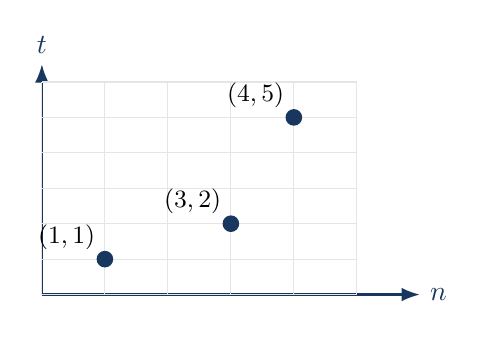
\begin{tikzpicture}[x=.8cm,y=.45cm]
\draw[ar] (0,0)--(6,0) node[right] {$n$};
\draw[ar] (0,0)--(0,6.5) node[above] {$t$};
\draw[gray!20,step=1] (0,0) grid (5,6);
\foreach \x/\y in {1/1,3/2,4/5}{
\fill[AcademicBlue] (\x,\y) circle (3pt);
\node[above left,font=\small] at (\x,\y) {$(\x,\y)$};}
\end{tikzpicture}\end{center}
Sumbu horizontal adalah eksponen $\gamma$, sumbu vertikal eksponen $\delta$.

\source{\S21.5, Gambar 21.6, hlm. 443--444; gambar digambar ulang}

\end{frame}
\begin{frame}{Mengapa perlu kuosien, bukan hanya himpunan titik?}

Himpunan titik bebas belum mengkodekan sifat dater yang tidak menurun.
Batas kuat pada kejadian awal otomatis memberi batas lebih lemah pada kejadian berikutnya.
\begin{block}{Penutupan tenggara}
Untuk $S\subseteq\mathbb Z^2$, definisikan
\[
\operatorname{cl}(S)=
\{(n+\kappa,t-\tau):(n,t)\in S,\ \kappa,\tau\in\N_0\}.
\]
\end{block}
Dua representasi dianggap ekuivalen jika penutupan tenggaranya sama.
Dioid kelas ekuivalensi tersebut adalah $\D$.
\medskip

Kita menghitung menggunakan titik pembangkit dan membuang kendala redundan.

\source{\S21.5, hlm. 444; konstruksi dijabarkan}
\end{frame}
\begin{frame}{Dominasi: kendala mana yang lebih kuat?}


Pada dioid hasil kuosien:
\[
\gamma^n\delta^t\oplus\gamma^{n+\kappa}\delta^{t-\tau}
=\gamma^n\delta^t,\qquad\kappa,\tau\ge0.
\]
Suku pertama mendominasi suku kedua.
\begin{exampleblock}{Contoh}
\[
\gamma\delta^4\oplus\gamma^3\delta^2=\gamma\delta^4.
\]
\end{exampleblock}
Jika kejadian kedua paling awal pada waktu $4$, maka kejadian keempat
tidak perlu diberi batas tambahan yang lebih lemah berupa waktu $2$.
Monotonisitas waktu kejadian membuat batas kedua redundan.

\source{\S21.5, hlm. 444}

\end{frame}
\begin{frame}{Ilustrasi kerucut tenggara}


\begin{center}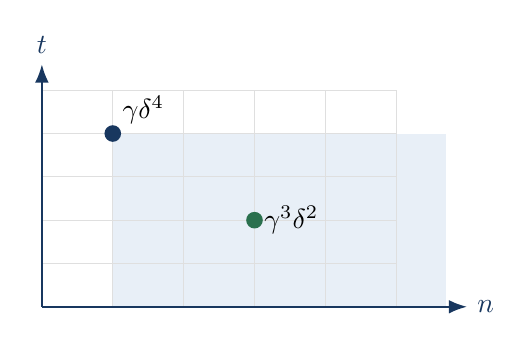
\begin{tikzpicture}[x=.9cm,y=.55cm]
\fill[SoftBlue] (1,0) rectangle (5.7,4);
\draw[gray!25,step=1] (0,0) grid (5,5);
\draw[ar] (0,0)--(6,0) node[right] {$n$};
\draw[ar] (0,0)--(0,5.6) node[above] {$t$};
\fill[AcademicBlue] (1,4) circle (3pt);
\node[above right] at (1,4) {$\gamma\delta^4$};
\fill[SolutionGreen] (3,2) circle (3pt);
\node[right] at (3,2) {$\gamma^3\delta^2$};
\end{tikzpicture}\end{center}
Daerah berwarna adalah potongan kerucut pada jendela gambar.
Kerucut sebenarnya berlanjut ke kanan dan ke bawah.
Titik $(3,2)$ sudah tercakup oleh titik $(1,4)$.

\source{\S21.5, Gambar 21.7, hlm. 444--445; ilustrasi kuliah}

\end{frame}
\begin{frame}{Aturan dasar operasi monomial}


\begin{align*}
\gamma^n\delta^t\oplus\gamma^\ell\delta^t
&=\gamma^{\min(n,\ell)}\delta^t,\\
\gamma^n\delta^t\oplus\gamma^n\delta^\tau
&=\gamma^n\delta^{\max(t,\tau)},\\
(\gamma^n\delta^t)(\gamma^\ell\delta^\tau)
&=\gamma^{n+\ell}\delta^{t+\tau}.
\end{align*}
\begin{block}{Batas penggunaan aturan}
Jika kedua eksponen berbeda, jumlah dua monomial dapat tetap terdiri dari dua suku.
Tidak selalu boleh mengambil minimum dan maksimum secara terpisah.
\end{block}

\source{\S21.5, hlm. 444; pers. (22.19)--(22.21), hlm. 458}

\end{frame}
\begin{frame}{Penurunan aturan penjumlahan khusus}

Jika waktu sama, indeks lebih kecil memberi kendala lebih kuat:
\[
\gamma^2\delta^5\oplus\gamma^4\delta^5=\gamma^2\delta^5.
\]
Jika indeks sama, waktu lebih besar memberi kendala lebih kuat:
\[
\gamma^2\delta^3\oplus\gamma^2\delta^7=\gamma^2\delta^7.
\]
\begin{exampleblock}{Hubungan dengan nama dioid}
Minimum muncul pada indeks kejadian yang sama waktunya.
Maksimum muncul pada waktu yang sama indeks kejadiannya.
\end{exampleblock}
Untuk pasangan dengan kedua koordinat berbeda, periksa dominasi terlebih dahulu.

\source{\S21.5, hlm. 440--445; \S22.2.3, hlm. 457--459}
\end{frame}
\begin{frame}{Contoh: jumlah yang tidak dapat dipadatkan}


Bandingkan
\[
a=\gamma\delta^2,\qquad b=\gamma^3\delta^5.
\]
$a$ memiliki indeks lebih kecil, tetapi waktu lebih kecil.
$b$ memiliki indeks lebih besar, tetapi waktu lebih besar.
\[
a\oplus b=\gamma\delta^2\oplus\gamma^3\delta^5.
\]
\begin{block}{Kesalahan yang perlu dihindari}
Mengganti jumlah ini dengan $\gamma\delta^5$ menambahkan kendala baru:
kejadian kedua harus menunggu sampai waktu $5$.
Kendala itu tidak berasal dari kedua suku semula.
\end{block}

\source{\S21.5; contoh kuliah}

\end{frame}
\begin{frame}{Urutan alami monomial}


Untuk eksponen hingga:
\[
\gamma^n\delta^t\preceq\gamma^\ell\delta^\tau
\quad\Longleftrightarrow\quad n\ge\ell\ \text{dan}\ t\le\tau.
\]
Artinya, suku kanan mendominasi suku kiri.
\begin{exampleblock}{Contoh}
\[
\gamma^3\delta^2\preceq\gamma\delta^4.
\]
Tetapi $\gamma\delta^2$ dan $\gamma^3\delta^5$ tidak dapat dibandingkan.
\end{exampleblock}
Identitas perkalian $e=\gamma^0\delta^0$ dan identitas penjumlahan $\eps$.
Dalam notasi batas buku, $\eps=\gamma^{+\infty}\delta^{-\infty}$.

\source{\S21.5, hlm. 444; \S22.2.3, hlm. 458}

\end{frame}
\begin{frame}{Polinomial dan bentuk kanonik}


Polinomial adalah jumlah berhingga monomial.
Untuk menyederhanakannya:
\begin{enumerate}
\item gabungkan suku dengan eksponen $\gamma$ yang sama;
\item buang suku yang didominasi suku lain;
\item urutkan suku yang tersisa berdasarkan eksponen $\gamma$.
\end{enumerate}
Bentuk kanonik mempunyai
\[
n_0<n_1<\cdots<n_r,\qquad t_0<t_1<\cdots<t_r.
\]
\begin{exampleblock}{Contoh}
\[
\gamma\delta\oplus\gamma^3\delta^2\oplus\gamma^4\delta^5
\oplus\gamma^5\delta^2
=\gamma\delta\oplus\gamma^3\delta^2\oplus\gamma^4\delta^5.
\]
\end{exampleblock}

\source{Contoh \S21.5; Definisi 22.7, hlm. 458}

\end{frame}
\begin{frame}{Perkalian polinomial: distribusi lalu reduksi}


Misalkan $p=\delta^2\oplus\gamma\delta^4$ dan
$q=\delta\oplus\gamma^2\delta^3$.
\begin{align*}
pq&=\delta^3\oplus\gamma^2\delta^5
\oplus\gamma\delta^5\oplus\gamma^3\delta^7\\
&=\delta^3\oplus\gamma\delta^5\oplus\gamma^3\delta^7.
\end{align*}
Suku $\gamma^2\delta^5$ didominasi oleh $\gamma\delta^5$.
\begin{block}{Prosedur}
Kalikan setiap pasangan suku, kemudian gunakan aturan dominasi.
Jumlah suku akhir dapat lebih kecil daripada hasil distribusi awal.
\end{block}

\source{Pers. (22.24)--(22.25); contoh kuliah}

\end{frame}
\begin{frame}{Infimum dua monomial}

Dalam urutan dioid, batas bawah terbesar dua monomial adalah
\[
\gamma^n\delta^t\wedge\gamma^\ell\delta^\tau
=\gamma^{\max(n,\ell)}\delta^{\min(t,\tau)}.
\]
\begin{exampleblock}{Contoh}
$(\gamma\delta^4)\wedge(\gamma^3\delta^2)=\gamma^3\delta^2$.\par\medskip
Untuk pasangan tidak terbandingkan:
\[
(\gamma\delta^2)\wedge(\gamma^3\delta^5)=\gamma^3\delta^2.
\]
\end{exampleblock}
Infimum berbeda dari jumlah $\oplus$, yang merupakan supremum.

\source{Pers. (22.23), hlm. 458}
\end{frame}
\begin{frame}{Dari satu place ke suku gamma--delta}


\begin{center}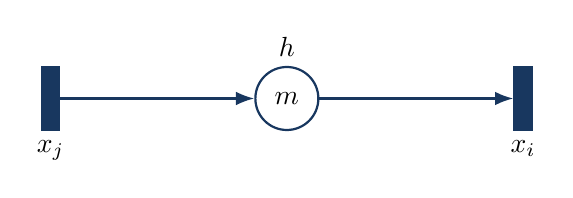
\begin{tikzpicture}
\node[tr,label=below:$x_j$] (a) at (0,0) {};
\node[pl,label=above:$h$] (p) at (3,0) {$m$};
\node[tr,label=below:$x_i$] (b) at (6,0) {};
\draw[ar] (a)--(p);\draw[ar] (p)--(b);
\end{tikzpicture}\end{center}
$m$ pada place menyatakan jumlah token awal.
\[
x_i(k)\ge h+x_j(k-m)
\quad\longleftrightarrow\quad
x_i\succeq\gamma^m\delta^h x_j.
\]
Jika ada beberapa prasyarat, gabungkan menggunakan $\oplus$.
Persamaan menyatakan perilaku paling awal dengan kondisi awal yang sesuai.

\source{\S21.1 dan \S21.5; skema kuliah}

\end{frame}
\begin{frame}{Prosedur sistematis membangun model TEG}

\begin{enumerate}
\item Beri nama dater untuk setiap transisi internal, input, dan output.
\item Untuk place dari $x_j$ ke $x_i$, catat token awal $m$ dan holding time $h$.
\item Tulis kontribusi $\gamma^m\delta^h x_j$ pada persamaan $x_i$.
\item Gabungkan seluruh input place menggunakan $\oplus$.
\item Susun matriks: pengaruh $x_j$ ke $x_i$ diletakkan pada $A_{ij}$.
\item Nyatakan kondisi awal dan pilih perilaku paling awal jika memakai persamaan.
\end{enumerate}
Place dengan $m=0,h=0$ memberi koefisien $e$, bukan $\eps$.
Tidak ada hubungan memberi koefisien $\eps$.

\source{\S21.5, hlm. 440--445; \S22.2.3, hlm. 457--459}
\end{frame}
\begin{frame}{Contoh satu mesin dengan kapasitas satu}


Masukan $u(k)$ adalah waktu kedatangan pekerjaan ke-$k$.
Mesin memerlukan $3$ satuan waktu dan hanya menangani satu pekerjaan.
\[
x(k)=\max\{u(k),x(k-1)+3\},\qquad y(k)=x(k)+3.
\]
$x$ adalah waktu mulai dan $y$ waktu selesai.
\[
x=\gamma\delta^3x\oplus u,\qquad y=\delta^3x.
\]
\begin{block}{Asumsi}
Urutan FIFO, mesin siap pada waktu $0$, dan $u(k)\ge0$.
Untuk rekursi, gunakan kondisi batas $x(0)=-3$.
\end{block}
Model sederhana ini akan digunakan kembali pada bagian kendali.

\source{\S21.5; model kuliah}

\end{frame}
\begin{frame}{TEG untuk mesin berkapasitas satu}

\begin{center}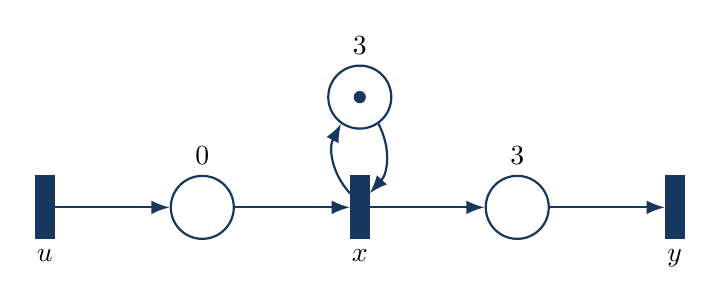
\begin{tikzpicture}
\node[tr,label=below:$u$] (u) at (0,0) {};
\node[tr,label=below:$x$] (x) at (4,0) {};
\node[tr,label=below:$y$] (y) at (8,0) {};
\node[pl,label=above:$0$] (p) at (2,0) {};
\node[pl,label=above:$3$] (q) at (6,0) {};
\node[pl,label=above:$3$] (r) at (4,1.4) {};\tok{r}
\draw[ar] (u)--(p);\draw[ar] (p)--(x);
\draw[ar] (x)--(q);\draw[ar] (q)--(y);
\draw[ar] (x) to[bend left=35] (r);
\draw[ar] (r) to[bend left=35] (x);
\end{tikzpicture}\end{center}
Angka luar place adalah holding time. Token loop mula-mula siap pada $0$.
\[
x=\gamma\delta^3x\oplus u,\qquad y=\delta^3x.
\]
Input $u$ mewakili kejadian eksogen; waktu firing-nya ditentukan dari luar model.

\source{Konstruksi kuliah dari \S21.5}
\end{frame}
\begin{frame}{Hitungan waktu pada contoh mesin}


Ambil $u(1)=0,\ u(2)=1,\ u(3)=7$, dengan $x(0)=-3$.
\begin{center}\begin{tabular}{c|rrr}\toprule
Pekerjaan $k$&1&2&3\\\midrule
Kedatangan $u(k)$&0&1&7\\
Mesin siap $x(k-1)+3$&0&3&6\\
Mulai $x(k)$&0&3&7\\
Selesai $y(k)$&3&6&10\\\bottomrule
\end{tabular}\end{center}
Pekerjaan kedua menunggu mesin. Pekerjaan ketiga menunggu kedatangannya sendiri.
\[
\gamma\delta^3
\]
menyimpan ketergantungan pada pekerjaan sebelumnya dan durasi $3$ sekaligus.


\end{frame}
\begin{frame}{Contoh buku: membaca hubungan lokal}

Pada TEG Gambar 21.5, hubungan menuju $x_1$ adalah:
\begin{center}\begin{tabular}{lrrl}\toprule
Dari&Token awal&Holding time&Suku\\\midrule
$u_1$&0&1&$\delta u_1$\\
$x_2$&1&4&$\gamma\delta^4x_2$\\\bottomrule
\end{tabular}\end{center}
Maka
\[
x_1=\delta u_1\oplus\gamma\delta^4x_2.
\]
Dalam dater:
\[
x_1(k)=\max\{u_1(k)+1,x_2(k-1)+4\}.
\]
Tabel hubungan lokal membantu memeriksa model satu persamaan demi satu.

\source{\S21.5, Gambar 21.5, hlm. 441--445}
\end{frame}
\begin{frame}{Contoh buku: tiga transisi internal}

\small

Model TEG pada Gambar 21.5:
\begin{align*}
x_1&=\gamma\delta^4x_2\oplus\delta u_1,\\
x_2&=\delta^3x_1\oplus\gamma\delta^5u_2,\\
x_3&=\delta^3x_1\oplus\delta^4x_2\oplus\gamma^2\delta^2x_3,\\
y&=\gamma x_2\oplus\delta^2x_3.
\end{align*}
\begin{exampleblock}{Membaca satu suku}
$\gamma^2\delta^2x_3$ berarti ketergantungan pada kejadian $x_3$
dua indeks sebelumnya dengan tambahan waktu $2$.
\end{exampleblock}
Tiga variabel cukup, dibandingkan delapan komponen pada pers. (21.18).

\source{\S21.5, hlm. 440--445}

\end{frame}
\begin{frame}{Representasi matriks contoh buku}


\[
x=Ax\oplus Bu,\qquad y=Cx,
\]
dengan
\[
A=\mpmat{\eps&\gamma\delta^4&\eps\\
\delta^3&\eps&\eps\\
\delta^3&\delta^4&\gamma^2\delta^2},
\qquad
B=\mpmat{\delta&\eps\\\eps&\gamma\delta^5\\\eps&\eps},
\]
\[
C=\mpmat{\eps&\gamma&\delta^2}.
\]
Baris $i$, kolom $j$ pada $A$ menyatakan pengaruh $x_j$ terhadap $x_i$.
Dimensi: $x\in D^3,\ u\in D^2,\ y\in D$ dengan $D=\D$.

\source{\S21.5, hlm. 444--445}

\end{frame}
\begin{frame}{Dari koefisien matriks kembali ke place}

Model $\D$ dapat dibaca kembali sebagai jaringan ketergantungan.
\begin{exampleblock}{Contoh}
Entri $A_{32}=\delta^4$ menyatakan:
\begin{itemize}
\item transisi produsen $x_2$, konsumen $x_3$;
\item satu place dengan holding time $4$;
\item tidak ada token awal pada place tersebut.
\end{itemize}
\end{exampleblock}
Entri $A_{33}=\gamma^2\delta^2$ menyatakan place loop dengan dua token awal dan holding time $2$.
\medskip

Jika suatu entri adalah jumlah beberapa monomial, masing-masing dapat mewakili ketergantungan paralel.

\source{\S21.5, hlm. 440--445; \S22.2.3, hlm. 457--459}
\end{frame}
\begin{frame}{Latihan: polinomial dan pemodelan}


\begin{enumerate}
\item Sederhanakan
$p=\gamma\delta^3\oplus\gamma^2\delta
\oplus\gamma^3\delta^6\oplus\gamma^4\delta^4$.
\item Hitung $(\delta^2\oplus\gamma\delta^4)\gamma^2\delta$.
\item Tuliskan model gamma--delta dari
\[
x(k)=\max\{u(k)+2,x(k-1)+4\},\qquad y(k)=x(k)+1.
\]
\item Jelaskan arti $\gamma^2\delta^7$ sebagai titik event--time dan sebagai operator.
\end{enumerate}
 


\end{frame}
\begin{frame}{Pembahasan: polinomial dan pemodelan}


\begin{enumerate}
\item $\gamma^2\delta$ didominasi oleh $\gamma\delta^3$ dan
$\gamma^4\delta^4$ oleh $\gamma^3\delta^6$:
\[
p=\gamma\delta^3\oplus\gamma^3\delta^6.
\]
\item Hasilnya $\gamma^2\delta^3\oplus\gamma^3\delta^5$.
\item $x=\delta^2u\oplus\gamma\delta^4x$, $y=\delta x$.
\item Titik: batas waktu paling awal $7$ untuk kejadian ketiga.
Operator: $(\gamma^2\delta^7x)(k)=x(k-2)+7$.
\end{enumerate}
\begin{block}{Bagian berikutnya}
Bagaimana menyelesaikan persamaan implisit $x=Ax\oplus Bu$?
\end{block}


\end{frame}
\begin{frame}{Persamaan implisit dan residuasi}
\begin{center}{\LARGE\bfseries\color{AcademicBlue}Persamaan implisit dan residuasi}\\[8mm]Solusi paling awal dan masukan paling lambat\end{center}
\end{frame}
\begin{frame}{Kelengkapan dioid dan penjumlahan tak hingga}


Dioid lengkap mendukung jumlah atas sembarang keluarga elemen,
dan perkalian distributif terhadap jumlah tersebut.
\[
\bigoplus_{n\ge0}a_n
\]
berarti supremum terhadap urutan alami dioid.
\begin{block}{Mengapa diperlukan?}
Sistem dapat mengulangi suatu siklus berapa kali pun.
Representasi semua pengulangan memerlukan deret tak hingga.
\end{block}
Pada max-plus lengkap, supremum dapat bernilai $+\infty$.
Pada dioid deret, pengulangan direpresentasikan secara simbolik.

\source{\S21.3, hlm. 437; \S22.2.2}

\end{frame}
\begin{frame}{Operator Kleene star}


\[
a^*=e\oplus a\oplus a^2\oplus a^3\oplus\cdots,
\qquad a^0=e.
\]
Untuk monomial $r=\gamma\delta^3$:
\[
r^*=e\oplus\gamma\delta^3
\oplus\gamma^2\delta^6\oplus\gamma^3\delta^9\oplus\cdots.
\]
\begin{exampleblock}{Interpretasi}
Setiap pengulangan menambahkan satu pergeseran kejadian dan tiga satuan waktu.
\end{exampleblock}
Pangkat di sini menggunakan perkalian dioid.

\source{Definisi 22.3, hlm. 455}

\end{frame}
\begin{frame}{Persamaan implisit dan solusi terkecil}


Pada dioid lengkap:
\[
x=ax\oplus b
\quad\Longrightarrow\quad
x_{\min}=a^*b.
\]
\textbf{Bukti bahwa kandidat adalah solusi}:
\[
a(a^*b)\oplus b=(aa^*\oplus e)b=a^*b.
\]
\textbf{Bukti minimalitas}: setiap solusi memenuhi $x\succeq b$, lalu
$x\succeq ab$, $x\succeq a^2b$, dan seterusnya. Maka
\[
x\succeq\bigoplus_{n\ge0}a^nb=a^*b.
\]
Solusi terkecil menggambarkan perilaku paling awal.

\source{Teorema 22.3, hlm. 455; bukti dijabarkan}

\end{frame}
\begin{frame}{Iterasi untuk membangun solusi terkecil}

Mulai dari elemen terkecil:
\[
x^{(0)}=\eps,\qquad x^{(r+1)}=ax^{(r)}\oplus b.
\]
Maka
\[
x^{(1)}=b,\quad x^{(2)}=ab\oplus b,\quad
x^{(3)}=a^2b\oplus ab\oplus b.
\]
Pada dioid lengkap:
\[
\bigoplus_{r\ge0}x^{(r)}=a^*b.
\]
Superskrip $(r)$ adalah nomor iterasi, bukan indeks firing $k$.
\begin{block}{Keterkaitan dengan titik tetap}
Kita mencari titik tetap operator monoton $F(x)=ax\oplus b$.
\end{block}

\source{\S22.2.2, hlm. 455; penjabaran konstruktif}
\end{frame}
\begin{frame}{Beberapa identitas Kleene star}

\[
a^*a^*=a^*,\qquad (a^*)^*=a^*,\qquad
a(ba)^*=(ab)^*a.
\]
Untuk dua elemen:
\[
(a\oplus b)^*=(a^*b)^*a^*=a^*(ba^*)^*.
\]
\begin{exampleblock}{Mengapa $a^*a^*=a^*$?}
Distribusi menghasilkan semua produk $a^ia^j=a^{i+j}$.
Semua pangkat tak negatif sudah ada pada $a^*$;
pengulangan suku hilang karena idempotensi.
\end{exampleblock}
Identitas ini berlaku pada dioid lengkap, termasuk matriks persegi berukuran sesuai.

\source{Properti 22.4, hlm. 456}
\end{frame}
\begin{frame}{Bentuk matriks dan fungsi transfer}


Untuk matriks pada dioid lengkap:
\[
A^*=E\oplus A\oplus A^2\oplus\cdots.
\]
Dari $x=Ax\oplus Bu$ dan $y=Cx$, pilih solusi terkecil:
\[
x=A^*Bu,\qquad y=Hu,\qquad H=CA^*B.
\]
\begin{block}{Interpretasi}
$H$ merangkum seluruh jalur pengaruh masukan ke keluaran,
termasuk pengulangan melalui siklus.
\end{block}
Tidak diperlukan invers matriks biasa $(I-A)^{-1}$.

\source{Pers. (22.32)--(22.33), hlm. 459--460}

\end{frame}
\begin{frame}{Arti fungsi transfer sebagai himpunan jalur}

Untuk setiap $r\ge0$:
\[
CA^rB
\]
merangkum pengaruh input ke output melalui $r$ hubungan internal.
\[
H=CB\oplus CAB\oplus CA^2B\oplus\cdots.
\]
\begin{exampleblock}{Pada aljabar gamma--delta}
Perkalian sepanjang jalur menjumlahkan token awal dan holding time.
Penjumlahan antarlintasan menggabungkan prasyarat waktu dan menghapus yang redundan.
\end{exampleblock}
Siklus menyebabkan deret tak hingga, tetapi sering dapat disimpan dengan Kleene star.

\source{\S22.2.2--22.3.1}
\end{frame}
\begin{frame}{Fungsi transfer mesin berkapasitas satu}


Model bagian sebelumnya:
\[
x=\gamma\delta^3x\oplus u,\qquad y=\delta^3x.
\]
Dengan solusi paling awal,
\[
x=(\gamma\delta^3)^*u,\qquad
H=\delta^3(\gamma\delta^3)^*.
\]
Ekspansinya:
\[
H=\delta^3\oplus\gamma\delta^6
\oplus\gamma^2\delta^9\oplus\cdots.
\]
Untuk pekerjaan ke-$k$:
\[
y(k)=\max_{1\le i\le k}\{u(i)+3(k-i+1)\}.
\]
Rumus ini berlaku untuk pekerjaan berindeks $1,2,\ldots$,
masukan nonnegatif, dan mesin mula-mula siap pada waktu $0$.

\source{\S22.2.2; contoh kuliah}

\end{frame}
\begin{frame}{Deret periodik dan laju asimtotik}


Buku menggunakan bentuk
\[
s=p\oplus qr^*,\qquad r=\gamma^\nu\delta^\tau,\quad\nu,\tau>0,
\]
dengan $p,q$ polinomial.
\begin{itemize}
\item $p$: bagian awal atau transien.
\item $qr^*$: bagian yang berulang.
\item Setiap pengulangan menambah $\nu$ kejadian dalam $\tau$ satuan waktu.
\end{itemize}
Buku mendefinisikan $\sigma_\infty(s)=\nu/\tau$.
\begin{exampleblock}{Mesin berkapasitas satu}
$H=\delta^3(\gamma\delta^3)^*$ memiliki laju asimtotik $1/3$
pekerjaan per satuan waktu dan waktu siklus $3$.
\end{exampleblock}

\source{Definisi 22.5, hlm. 457}

\end{frame}
\begin{frame}{Deret periodik dengan bagian transien}

Misalkan
\[
s=\delta^2\oplus\gamma\delta^5
\oplus\gamma^2\delta^9(\gamma\delta^3)^*.
\]
Ekspansinya:
\[
s=\delta^2\oplus\gamma\delta^5\oplus\gamma^2\delta^9
\oplus\gamma^3\delta^{12}\oplus\gamma^4\delta^{15}\oplus\cdots.
\]
\begin{itemize}
\item Bagian awal: $\delta^2\oplus\gamma\delta^5$.
\item Bagian berulang mulai pada $\gamma^2\delta^9$.
\item Selanjutnya, tambahan satu indeks memerlukan tambahan waktu $3$.
\end{itemize}
Laju asimtotiknya $\sigma_\infty=1/3$.

\source{Definisi 22.5, hlm. 457; contoh kuliah}
\end{frame}
\begin{frame}{Mengapa memerlukan residuasi?}


Untuk mengejar tenggat $z$, kita ingin memilih masukan selambat mungkin:
\[
Hu\preceq z.
\]
Persamaan $Hu=z$ mungkin tidak mempunyai solusi.
\begin{block}{Residuasi}
Untuk pemetaan monoton $L_H:u\mapsto Hu$ yang residuated:
\[
H\res z=\max_{\preceq}\{u:Hu\preceq z\}.
\]
\end{block}
Ini adalah solusi terbesar pertidaksamaan, bukan invers biasa.
Untuk perkalian pada dioid lengkap, residuasi menyediakan konstruksi tersebut.

\source{\S22.2.1, hlm. 453--454; \S22.3.1}

\end{frame}
\begin{frame}{Pemetaan residuated dan sifat adjungsi}

Pemetaan monoton $f:D\to C$ disebut residuated jika
\[
f^\sharp(b)=\max_{\preceq}\{x:f(x)\preceq b\}
\]
ada untuk setiap $b\in C$.
Sifat utamanya:
\[
f(x)\preceq b\quad\Longleftrightarrow\quad x\preceq f^\sharp(b).
\]
Akibat langsung:
\[
f(f^\sharp(b))\preceq b,\qquad x\preceq f^\sharp(f(x)).
\]
Pada dioid lengkap, residu perkalian kiri ditulis $a\res b$.
Residu perkalian kanan ditulis $b/\!^\circ a$.

\source{Definisi 22.1--22.2, Teorema 22.1, hlm. 453}
\end{frame}
\begin{frame}{Mengapa residuasi memberi solusi terbesar?}

Misalkan $u_{\rm opt}=H\res z$.
\begin{enumerate}
\item Kelayakan: $Hu_{\rm opt}\preceq z$.
\item Untuk masukan feasible lain $v$, berlaku $Hv\preceq z$.
\item Sifat adjungsi memberi $v\preceq H\res z=u_{\rm opt}$.
\end{enumerate}
\begin{block}{Arti optimalitas}
Tidak ada masukan feasible yang lebih besar dalam urutan dioid.
Pada dater max-plus, lebih besar berarti waktu pelepasan lebih lambat.
\end{block}
Optimalitas ini menggunakan model, data tenggat, dan himpunan masukan yang telah ditetapkan.

\source{\S22.2.1 dan \S22.3.1}
\end{frame}
\begin{frame}{Residuasi skalar max-plus}


Untuk $a,b$ hingga:
\[
a\otimes u\preceq b
\quad\Longleftrightarrow\quad
a+u\le b
\quad\Longleftrightarrow\quad
u\le b-a.
\]
Maka $a\res b=b-a$.
\begin{exampleblock}{Contoh}
Durasi proses $5$, tenggat $12$:
\[
5\otimes u\le12\quad\Longrightarrow\quad u_{\mathrm{opt}}=7.
\]
\end{exampleblock}
Pengurangan ini berlaku untuk residuasi skalar hingga.
Untuk matriks, setiap komponen masukan harus memenuhi semua kendala keluaran.

\source{\S22.2.1, hlm. 454}

\end{frame}
\begin{frame}{Residuasi matriks max-plus}


Untuk $A$ dan $z$ berhingga:
\[
A\otimes u\preceq z
\quad\Longleftrightarrow\quad
A_{ij}+u_j\le z_i\quad\text{untuk semua }i,j.
\]
Karena itu,
\[
u_j^{\mathrm{opt}}=\min_i(z_i-A_{ij}).
\]
Jika $A_{ij}=\eps=-\infty$, kendala tersebut tidak membatasi $u_j$.
\begin{block}{Makna}
Maksimum menyatukan waktu kesiapan keluaran.
Minimum menyatukan semua batas atas yang harus dipenuhi masukan.
\end{block}

\source{Pers. (22.4), hlm. 454; penjabaran max-plus}

\end{frame}
\begin{frame}{Contoh residuasi matriks dari buku}


\[
A=\mpmat{2&5\\\eps&3\\0&7},\qquad z=\mpmat{6\\4\\9}.
\]
\[
u_{\mathrm{opt}}=
\mpmat{\min(6-2,+\infty,9-0)\\
\min(6-5,4-3,9-7)}
=\mpmat{4\\1}.
\]
Verifikasi:
\[
A\otimes u_{\mathrm{opt}}=\mpmat{6\\4\\8}
\preceq\mpmat{6\\4\\9}.
\]
Keluaran ketiga lebih awal dari tenggat. Residuasi tidak menjamin persamaan tepat.

\source{Contoh 22.2, hlm. 454}

\end{frame}
\begin{frame}{Residuasi monomial gamma--delta}


Untuk monomial dengan eksponen hingga, pada dioid penuh:
\[
(\gamma^n\delta^t)\res(\gamma^\ell\delta^\tau)
=\gamma^{\ell-n}\delta^{\tau-t}.
\]
\begin{exampleblock}{Contoh}
\[
(\gamma\delta^3)\res(\gamma^2\delta^{10})
=\gamma\delta^7.
\]
Periksa:
\[
(\gamma\delta^3)(\gamma\delta^7)=\gamma^2\delta^{10}.
\]
\end{exampleblock}
Residuasi dapat menghasilkan eksponen negatif.
Untuk kendali yang dapat diimplementasikan, kausalitas perlu diperiksa.

\source{Pers. (22.22), hlm. 458; contoh kuliah}

\end{frame}
\begin{frame}{Residuasi polinomial: menggabungkan semua kendala}

Jika $a=\bigoplus_i a_i$, maka
\[
a\res b=\bigwedge_i(a_i\res b).
\]
Sebab $ax\preceq b$ harus berlaku untuk setiap kontribusi $a_ix$.
\begin{exampleblock}{Contoh}
Untuk $a=e\oplus\gamma\delta^3$ dan $b=\gamma^2\delta^8$:
\[
a\res b=(\gamma^2\delta^8)\wedge(\gamma\delta^5)
=\gamma^2\delta^5.
\]
\end{exampleblock}
Periksa $a(\gamma^2\delta^5)
=\gamma^2\delta^5\oplus\gamma^3\delta^8\preceq\gamma^2\delta^8$.

\source{Pers. (22.27), hlm. 458; contoh kuliah}
\end{frame}
\begin{frame}{Kausalitas: definisi dan interpretasi}

Untuk deret tak nol $s$ dengan valuasi hingga,
$\operatorname{val}(s)$ adalah eksponen $\gamma$ terkecil pada dukungannya.
Buku mendefinisikan kausalitas melalui
\[
\operatorname{val}(s)\ge0,\qquad
s\succeq\gamma^{\operatorname{val}(s)}.
\]
Deret nol $\eps$ juga kausal.
\begin{exampleblock}{Polinomial kanonik}
Jika eksponen pertama $(n_0,t_0)$ memenuhi $n_0\ge0$ dan $t_0\ge0$,
semua suku berikutnya mempunyai eksponen nonnegatif.
\end{exampleblock}
Operator dengan pangkat $\gamma$ negatif dapat memerlukan kejadian masa depan;
pangkat $\delta$ negatif merepresentasikan pergeseran waktu negatif.

\source{Definisi 22.4, hlm. 457}
\end{frame}
\begin{frame}{Realisasi dan proyeksi ke deret kausal}

Untuk kelas deret periodik yang dibahas buku:
\[
s\text{ dapat direalisasikan oleh TEG}
\quad\Longleftrightarrow\quad
s\text{ periodik dan kausal}.
\]
Proyeksi $\operatorname{Pr}_+(s)$ adalah deret kausal terbesar yang memenuhi
$\operatorname{Pr}_+(s)\preceq s$.
\begin{exampleblock}{Contoh polinomial kanonik}
\[
s=\gamma^{-1}\delta^2\oplus\delta^4
\quad\Longrightarrow\quad
\operatorname{Pr}_+(s)=\delta^4.
\]
\end{exampleblock}
Untuk representasi umum, gunakan penutupan dan bentuk kanonik sebelum
menafsirkan suku. Proyeksi bukan sekadar mengganti pangkat negatif menjadi nol.

\source{Teorema 22.6--22.7, hlm. 458--459}
\end{frame}
\begin{frame}{Kendali dan pemeriksaan spesifikasi}
\begin{center}{\LARGE\bfseries\color{AcademicBlue}Kendali dan pemeriksaan spesifikasi}\\[8mm]Dari batas keluaran ke jadwal masukan\end{center}
\end{frame}
\begin{frame}{Kendali just-in-time}


Dengan $H=CA^*B$, tujuan kendali adalah
\[
u_{\mathrm{opt}}=H\res z,\qquad
y_{\mathrm{opt}}=Hu_{\mathrm{opt}}\preceq z.
\]
\begin{itemize}
\item $z$: tenggat keluaran yang diketahui sebelumnya.
\item $u_{\mathrm{opt}}$: masukan selambat mungkin yang tetap memenuhi tenggat.
\item $y_{\mathrm{opt}}$: keluaran yang benar-benar dapat dicapai.
\end{itemize}
\begin{block}{Interpretasi}
Kendali menunda pelepasan pekerjaan. Kendali tidak mempersingkat durasi fisik proses.
\end{block}

\source{\S22.1, hlm. 451--452; \S22.3.1, hlm. 459--460}

\end{frame}
\begin{frame}{Contoh kendali: tiga pekerjaan pada satu mesin}


Mesin membutuhkan $3$ satuan waktu per pekerjaan.
Tenggat tiga keluaran adalah
\[
z(1)=5,\quad z(2)=7,\quad z(3)=12.
\]
Untuk $i\le k$:
\[
u(i)+3(k-i+1)\le z(k).
\]
Maka
\[
u_{\mathrm{opt}}(i)=\min_{k=i,\ldots,3}
\{z(k)-3(k-i+1)\}.
\]
\begin{block}{Asumsi contoh}
Seluruh tenggat diketahui, pekerjaan tersedia untuk dilepas,
urutan FIFO, dan mesin siap pada waktu $0$.
\end{block}

\source{\S22.3.1; contoh kuliah berdasarkan model mesin}

\end{frame}
\begin{frame}{Perhitungan jadwal masukan paling lambat}


\begin{align*}
u_{\mathrm{opt}}(1)&=\min(5-3,\ 7-6,\ 12-9)=1,\\
u_{\mathrm{opt}}(2)&=\min(7-3,\ 12-6)=4,\\
u_{\mathrm{opt}}(3)&=12-3=9.
\end{align*}
Jadi $u_{\mathrm{opt}}=(1,4,9)$.
\begin{exampleblock}{Mengapa pekerjaan pertama tidak boleh masuk pada $2$?}
Pekerjaan pertama selesai pada $5$, sehingga pekerjaan kedua paling awal
selesai pada $8$. Tenggat kedua adalah $7$.
\end{exampleblock}
Tenggat pekerjaan berikutnya dapat membatasi waktu pelepasan pekerjaan sebelumnya.


\end{frame}
\begin{frame}{Verifikasi jadwal terhadap spesifikasi}


Dengan $x(0)=-3$ dan $x(k)=\max\{u(k),x(k-1)+3\}$:
\begin{center}\begin{tabular}{c|rrr}\toprule
Pekerjaan&1&2&3\\\midrule
Masukan $u(k)$&1&4&9\\
Mulai $x(k)$&1&4&9\\
Selesai $y(k)$&4&7&12\\
Tenggat $z(k)$&5&7&12\\
Slack $z(k)-y(k)$&1&0&0\\\bottomrule
\end{tabular}\end{center}
Semua memenuhi $y(k)\le z(k)$.
\begin{block}{Hubungan dengan verifikasi formal}
Spesifikasi waktu menjadi pertidaksamaan matematis.
Residuasi menyintesis masukan, lalu model memeriksa kepatuhannya.
\end{block}


\end{frame}
\begin{frame}{Kelayakan dan batas fisik sistem}

Untuk mesin durasi $3$, siap pada $0$, dan masukan $u(1)\ge0$:
\[
y(1)\ge3.
\]
Tenggat $z(1)=2$ tidak feasible.
Residuasi tanpa batas pelepasan memberi $u(1)\le-1$,
tetapi nilai ini tidak diperbolehkan oleh asumsi.
\begin{block}{Prosedur pemeriksaan}
Hitung kendala, lalu periksa kembali batas pelepasan,
keadaan awal, dan urutan pekerjaan.
\end{block}
Jika terdapat batas bawah masukan $\underline u$, kelayakan memerlukan
$\underline u\preceq H\res z$.

\source{\S22.3.1; pembatasan tambahan pada contoh kuliah}
\end{frame}
\begin{frame}{Latihan: fungsi transfer dan just-in-time}


\begin{enumerate}
\item Selesaikan $x=\gamma\delta^2x\oplus\delta u$ dan $y=\delta x$
dalam bentuk fungsi transfer $y=Hu$.
\item Tuliskan tiga monomial pertama $H$.
\item Untuk mesin durasi $2$ yang mula-mula siap pada $0$,
tentukan masukan paling lambat bagi tenggat $z=(4,5,9)$.
\item Verifikasi waktu keluarannya.
\end{enumerate}
Soal 3--4 memakai model mesin $y(k)=\max\{u(k)+2,y(k-1)+2\}$
dengan $y(0)=0$.
 


\end{frame}
\begin{frame}{Pembahasan: fungsi transfer dan just-in-time}


\[
H=\delta^2(\gamma\delta^2)^*
=\delta^2\oplus\gamma\delta^4\oplus\gamma^2\delta^6\oplus\cdots.
\]
Untuk mesin durasi $2$ dan $z=(4,5,9)$:
\begin{align*}
u_{\mathrm{opt}}(1)&=\min(4-2,5-4,9-6)=1,\\
u_{\mathrm{opt}}(2)&=\min(5-2,9-4)=3,\\
u_{\mathrm{opt}}(3)&=9-2=7.
\end{align*}
Dengan $y(0)=0$:
\[
y(1)=3,\qquad y(2)=5,\qquad y(3)=9.
\]
Jadi $y=(3,5,9)\le(4,5,9)$.


\end{frame}
\begin{frame}{Filter dan umpan balik}
\begin{center}{\LARGE\bfseries\color{AcademicBlue}Filter dan umpan balik}\\[8mm]Kendali berdasarkan model referensi\end{center}
\end{frame}
\begin{frame}{Filter masukan dan model referensi}

Sistem asli: $y=Hu$.
Model referensi: $z=Gv$.
Gunakan filter $u=Pv$.
\[
y=HPv.
\]
Agar $y\preceq z$ untuk semua masukan model $v$, gunakan syarat
\[
HP\preceq G.
\]
\begin{block}{Sintesis filter}
\[
P_{\rm opt}=H\res G.
\]
\end{block}
Jika diperlukan filter kausal, gunakan $\operatorname{Pr}_+(P_{\rm opt})$.

\source{\S22.3.2, pers. (22.40)--(22.42), hlm. 462}
\end{frame}
\begin{frame}{Ilustrasi arsitektur filter}

\begin{center}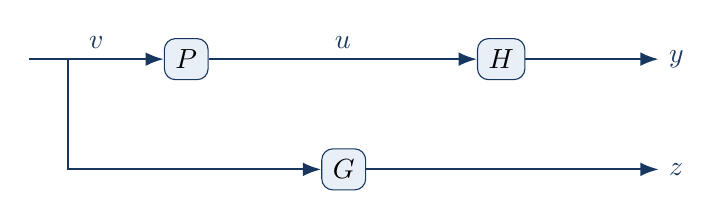
\begin{tikzpicture}
\node[state] (p) at (2,0) {$P$};
\node[state] (h) at (6,0) {$H$};
\draw[ar] (0,0)--node[above]{$v$}(p);
\draw[ar] (p)--node[above]{$u$}(h);
\draw[ar] (h)--(8,0) node[right]{$y$};
\node[state] (g) at (4,-1.4) {$G$};
\draw[ar] (.5,0)--(.5,-1.4)--(g);
\draw[ar] (g)--(8,-1.4) node[right]{$z$};
\end{tikzpicture}\end{center}
Cabang bawah menentukan perilaku referensi.
Cabang atas menghasilkan perilaku sistem setelah filter.
\[
HP\preceq G\quad\Longrightarrow\quad HPv\preceq Gv.
\]
Dimensi filter harus sesuai dengan banyaknya input sistem dan input referensi.

\source{\S22.3.2; diagram penjelas}
\end{frame}
\begin{frame}{Filter netral: keluaran tetap, masukan ditunda}

Pilih referensi $G=H$. Maka
\[
P_{\rm opt}=H\res H,\qquad HP_{\rm opt}=H.
\]
\begin{exampleblock}{Mengapa persamaan berlaku?}
$E$ feasible karena $HE=H$, sehingga $E\preceq P_{\rm opt}$.
Monotonisitas memberi $H\preceq HP_{\rm opt}$.
Kelayakan memberi $HP_{\rm opt}\preceq H$.
\end{exampleblock}
Jadi filter dapat menunda masukan tanpa menunda keluaran.
Tujuannya mengurangi waktu tunggu internal dan persediaan dalam proses.
Kesimpulan menggunakan model yang diasumsikan tepat.

\source{Pers. (22.43), hlm. 462--463}
\end{frame}
\begin{frame}{Contoh filter netral pada dua jalur sinkronisasi}

Gunakan $H=\mpmat{2&5}$ pada max-plus.
\[
P_{\rm opt}=H\res H
=\mpmat{0&3\\-3&0}.
\]
Untuk $v=(0,0)^T$:
\[
y_{\rm tanpa\ filter}=\max(2,5)=5,
\]
\[
u=P_{\rm opt}v=(3,0)^T,\qquad
y_{\rm filter}=\max(3+2,0+5)=5.
\]
Jalur pertama ditunda dari $0$ ke $3$, karena sebelumnya menunggu jalur kedua.
Ini contoh aljabar waktu hingga; bukan langsung realisasi filter gamma--delta kausal.

\source{\S22.3.2; contoh kuliah}
\end{frame}
\begin{frame}{Umpan balik keluaran}

Tambahkan kendali $F$ dari keluaran ke masukan:
\[
u=Fy\oplus Pv.
\]
Dengan $x=Ax\oplus Bu$ dan $y=Cx$:
\[
x=(A\oplus BFC)x\oplus BPv.
\]
Solusi terkecil:
\[
y=C(A\oplus BFC)^*BPv.
\]
Jika $H=CA^*B$, identitas Kleene star memberi
\[
y=H(FH)^*Pv.
\]
Umpan balik menambahkan ketergantungan dari kejadian keluaran ke kejadian masukan.

\source{\S22.3.3, pers. (22.49)--(22.52), hlm. 464--465}
\end{frame}
\begin{frame}{Sintesis umpan balik dalam buku}

Tujuan model matching adalah
\[
H(FH)^*P\preceq G.
\]
Buku terlebih dahulu memilih $P_{\rm opt}=H\res G$.
Untuk pilihan tersebut, batas terhadap $F$ dapat dinyatakan
\[
FH\preceq P_{\rm opt}/\!^\circ P_{\rm opt}.
\]
Maka solusi terbesar tanpa pembatasan kausal adalah
\[
F_{\rm opt}
=(P_{\rm opt}/\!^\circ P_{\rm opt})/\!^\circ H.
\]
Gunakan $F_{\rm opt}^{+}=\operatorname{Pr}_+(F_{\rm opt})$
untuk kendali kausal, bersama filter kausal yang sesuai.

\source{\S22.3.3, pers. (22.53)--(22.57), hlm. 465}
\end{frame}
\begin{frame}{Makna kendali umpan balik pada TEG}

Untuk satu jalur feedback, misalkan
\[
u=\gamma^2\delta^h y\oplus v.
\]
Dalam dater:
\[
u(k)=\max\{y(k-2)+h,v(k)\}.
\]
\begin{exampleblock}{Interpretasi}
Pelepasan pekerjaan ke-$k$ menunggu keluaran pekerjaan ke-$(k-2)$
beserta tambahan waktu $h$.
Dua token pada place feedback membatasi banyak pekerjaan yang belum selesai.
\end{exampleblock}
Makna tepat kapasitas dan kesiapan awal mengikuti definisi input/output
serta marking awal model.

\source{\S22.3.3; contoh kuliah}
\end{frame}
\begin{frame}{Studi kasus HTS}
\begin{center}{\LARGE\bfseries\color{AcademicBlue}Studi kasus HTS}\\[8mm]Contoh buku yang ditelusuri dari proses ke persamaan\end{center}
\end{frame}
\begin{frame}{High-throughput screening: urutan kegiatan}

Contoh buku menggunakan tiga sumber daya:
\begin{itemize}
\item $R_1$: mengisi zat A ke microplate, durasi $7$, lalu post-processing $1$.
\item $R_2$: persiapan $1$, menunggu sebelum penambahan B selama $1$,
kemudian mencampur selama $12$.
\item $R_3$: menyediakan zat B selama $5$, lalu post-processing $1$.
\end{itemize}
Transfer dianggap tanpa durasi.
\begin{block}{Kapasitas}
$R_1$ dan $R_3$ berkapasitas satu. $R_2$ berkapasitas dua.
Satu batch harus menyelaraskan microplate A dan ketersediaan zat B.
\end{block}

\source{\S21.6, hlm. 445--447}
\end{frame}
\begin{frame}{Arti sepuluh kejadian internal HTS}

\small
\begin{center}\begin{tabular}{cl}\toprule
Kejadian&Arti dalam model\\\midrule
$x_1,x_2,x_3$&Mulai pengisian A; selesai pengisian; selesai post-processing $R_1$\\[2mm]
$x_4,x_5$&Mulai persiapan $R_2$; transfer microplate dimungkinkan\\[2mm]
$x_6,x_7$&Mulai pencampuran; selesai pencampuran\\[2mm]
$x_8,x_9,x_{10}$&Mulai penyediaan B; B tersedia; selesai post-processing $R_3$\\\bottomrule
\end{tabular}\end{center}
Transfer mensinkronkan $x_2$ dan $x_5$ melalui dua kendala waktu nol.
Input $u_1,u_2,u_3$ memerintah awal kegiatan $x_1,x_4,x_8$.
Output $y$ mengikuti $x_7$.

\source{\S21.6, Gambar 21.8--21.10, hlm. 446--448}
\end{frame}
\begin{frame}{HTS: hubungan pada R1 dan R2}

\begin{align*}
x_1&=\gamma x_3\oplus u_1,\\
x_2&=\delta^7x_1\oplus x_5,\\
x_3&=\delta x_2,\\
x_4&=\gamma^2x_7\oplus u_2,\\
x_5&=\delta x_4\oplus x_2.
\end{align*}
\begin{itemize}
\item $\gamma x_3$: penggunaan kembali satu unit kapasitas $R_1$.
\item $\gamma^2x_7$: dua unit kapasitas $R_2$.
\item $x_2$ dan $x_5$: sinkronisasi transfer microplate.
\end{itemize}

\source{\S21.6, model matriks hlm. 448; ditulis per baris}
\end{frame}
\begin{frame}{HTS: pencampuran dan penyediaan B}\setlength{\jot}{1pt}

\begin{align*}
x_6&=\delta x_5\oplus x_9,\\
x_7&=\delta^{12}x_6,\\
x_8&=\gamma x_{10}\oplus u_3,\\
x_9&=\delta^5x_8,\qquad x_{10}=\delta x_9,\\
y&=x_7.
\end{align*}
Pencampuran $x_6$ menunggu kesiapan microplate dan zat B.
\begin{block}{Interpretasi sumber daya}
Token pada loop kapasitas membatasi overlap antarbatches.
Kapasitas tidak dimodelkan dengan mengubah bobot arc menjadi dua.
\end{block}

\source{\S21.6, model matriks hlm. 448; ditulis per baris}
\end{frame}
\begin{frame}{HTS: menghitung waktu satu batch}

Anggap sumber daya tersedia pada waktu $0$, $u_1=u_2=u_3=0$,
dan tidak ada batch terdahulu yang membatasi.
\[
x_1=x_4=x_8=0,\qquad x_9=5.
\]
Dari sinkronisasi transfer:
\[
x_2=\max(7,x_5),\qquad x_5=\max(1,x_2).
\]
Solusi paling awal adalah $x_2=x_5=7$. Maka
\[
x_3=8,\quad x_{10}=6,\quad
x_6=\max(7+1,5)=8,\quad y=x_7=20.
\]
Satu batch pertama selesai pada waktu $20$.

\source{Contoh perhitungan dari model \S21.6}
\end{frame}
\begin{frame}{HTS: kapasitas dan bottleneck antarbatches}

Tiga loop sumber daya memberi rata-rata waktu per batch:
\begin{center}\begin{tabular}{lccc}\toprule
Sumber daya&Waktu satu putaran&Token&Rata-rata\\\midrule
$R_1$&$7+1=8$&1&8\\
$R_2$&$1+1+12=14$&2&7\\
$R_3$&$5+1=6$&1&6\\\bottomrule
\end{tabular}\end{center}
Loop $R_1$ memberikan batas interval paling sedikit $8$.
\begin{block}{Analisis menyeluruh}
Sistem dapat mempunyai siklus lain akibat sinkronisasi.
Nilai akhir harus diperiksa dari seluruh graf atau fungsi transfer,
bukan hanya kapasitas lokal.
\end{block}
Pada fungsi transfer contoh buku, faktor periodiknya adalah $(\gamma\delta^8)^*$.

\source{\S21.6; pers. (22.36), hlm. 461}
\end{frame}
\begin{frame}{HTS: referensi keluaran dan hasil kendali buku}

Buku memberi referensi
\[
z=\delta^{37}\oplus\gamma\delta^{42}
\oplus\gamma^3\delta^{55}\oplus\gamma^4\delta^{+\infty}.
\]
Ini berarti tenggat empat keluaran dapat ditulis $(37,42,55,55)$.
Hasil kendali optimal buku memberi keluaran:
\[
y_{\rm opt}=(28,36,42,55).
\]
\begin{block}{Pemeriksaan}
$28\le37$, $36\le42$, $42\le55$, dan $55\le55$.
Sebagian keluaran lebih awal daripada referensi karena keterkaitan dinamika sistem.
\end{block}
Suku $\gamma^4\delta^{+\infty}$ mengakhiri horizon empat keluaran pada representasi tersebut.

\source{\S22.3.1.1, pers. (22.37)--(22.39), hlm. 461}
\end{frame}
\begin{frame}{Hubungan dengan verifikasi formal}

\begin{enumerate}
\item \textbf{Model}: TEG, kondisi awal, dan persamaan dioid.
\item \textbf{Spesifikasi}: tenggat, kapasitas, atau batas keterlambatan.
\item \textbf{Sintesis}: cari kendali yang membuat model memenuhi spesifikasi.
\item \textbf{Verifikasi}: periksa kendala untuk keluaran dan semua kondisi yang disyaratkan.
\end{enumerate}
\begin{block}{Batas jaminan}
Perhitungan membuktikan sifat model di bawah asumsi durasi,
kapasitas, dan ketersediaan yang digunakan.
Durasi tak pasti atau konflik memerlukan perluasan model dan analisis.
\end{block}

\end{frame}
\begin{frame}{Ringkasan hubungan antarrepresentasi}

\begin{center}\begin{tabular}{p{3cm}p{8.5cm}}\toprule
Representasi&Informasi yang ditonjolkan\\\midrule
Petri net&Kondisi, sumber daya, dan kejadian\\[1.5mm]
Event graph&Ketergantungan sinkronisasi tanpa konflik\\[1.5mm]
TEG&Jumlah token awal dan durasi ketergantungan\\[1.5mm]
Max-plus&Waktu kejadian dan evolusi rekursif\\[1.5mm]
$\D$&Pergeseran kejadian dan waktu secara simbolik\\[1.5mm]
$H=CA^*B$&Hubungan semua input dengan semua output\\[1.5mm]
$u_{\rm opt}=H\res z$&Masukan paling lambat yang memenuhi batas keluaran\\\bottomrule
\end{tabular}\end{center}

\end{frame}
\begin{frame}{Glosarium simbol}

\small
\begin{center}\begin{tabular}{ll}\toprule
$P,T,A_{\rm arc},w$&Place, transisi, arc, dan bobot arc Petri net\\
$m_0,h_p$&Marking awal dan holding time pada place\\
$x_i(k)$&Waktu kejadian ke-$k$ pada transisi $i$\\
$\eps,e$&Identitas penjumlahan dan perkalian dioid\\
$\oplus,\otimes$&Penjumlahan dan perkalian pada dioid yang dipilih\\
$\preceq,\wedge$&Urutan alami dan infimum\\
$\gamma,\delta$&Pergeseran indeks kejadian dan waktu\\
$A,B,C$&Matriks internal, masukan, dan keluaran sistem dioid\\
$A^*,H$&Kleene star matriks dan fungsi transfer\\
$a\res b,\ b/\!^\circ a$&Residu perkalian kiri dan kanan\\
$P_{\rm opt},F_{\rm opt}$&Filter dan kendali umpan balik optimal\\\bottomrule
\end{tabular}\end{center}
Simbol $A$ dan $P$ memiliki arti berbeda pada konteks Petri net dan kendali.

\end{frame}
\begin{frame}{Referensi utama}


\small
\begin{enumerate}
\item Seatzu, C., Silva, M., dan van Schuppen, J. H. (eds.) (2013).
\textit{Control of Discrete-Event Systems: Automata and Petri Net Perspectives}.
LNCIS 433, Springer. DOI: 10.1007/978-1-4471-4276-8.
\item Brunsch, T., Raisch, J., Hardouin, L., dan Boutin, O.
Bab 21: \textit{Discrete-Event Systems in a Dioid Framework: Modeling and Analysis},
hlm. 431--450.
\item Hardouin, L., Boutin, O., Cottenceau, B., Brunsch, T., dan Raisch, J.
Bab 22: \textit{Discrete-Event Systems in a Dioid Framework: Control Theory},
hlm. 451--469.
\end{enumerate}
Nomor halaman dalam slide mengikuti halaman cetak buku.
Contoh berlabel kuliah adalah penyederhanaan untuk pembelajaran.


\end{frame}
\begin{frame}{Petunjuk membaca ulang materi}

\begin{itemize}
\item Jika kesulitan pada rekursi waktu, ulangi enabling, holding time, dan peran token awal.
\item Jika kesulitan pada operasi simbolik, ulangi urutan alami dan dominasi monomial.
\item Jika kesulitan pada fungsi transfer, ulangi iterasi $x=ax\oplus b$.
\item Jika kesulitan pada kendali, tuliskan dahulu semua pertidaksamaan waktu dalam aritmetika biasa.
\end{itemize}
\begin{block}{Latihan mandiri lanjutan}
Ubah durasi mesin dari $3$ menjadi $4$.
Turunkan kembali model, fungsi transfer, dan jadwal just-in-time untuk tenggat yang dipilih sendiri.
\end{block}

\end{frame}
\end{document}
